\documentclass{book}

\usepackage{amsmath}
\usepackage{imakeidx}


\makeindex

\begin{document}

%%% frontmatter %%%
\frontmatter

\title{Angewandte Kryptographie}
\author{FH Campus Wien}
\date{SoSe 2025}

\maketitle
\tableofcontents

%%% mainmatter %%%
\mainmatter

\chapter{Effiziente Implementierungen}

%%% section %%%
\section{Langzahlen}

In (asymmetrischer) Kryptographie benötigen wir üblicherweise Werte, die weit größer sind als die native Wortlänge der zugrundeliegenden Hardware.
Die meisten Register haben eine Wortlänge von 64 bit. Typische Schlüssellängen, beispielsweise für RSA Verschlüsselung, sind heutzutage 1024 bis 4096 bits.

\paragraph{Wie können solche Zahlen dargestellt werden?}

Eine Auswahl an Möglichkeiten ist:

\begin{enumerate}
    \item Residuen-Repräsentation \index{Residuen-Repräsentation}
    \item Verwendung von Arrays in nativer Wortgröße \index{Arrays!mit nativer Wortgröße}
    \item Verwendung von Arrays kleiner als die native Wortgröße \index{Arrays!kleiner als die native Wortgröße}
\end{enumerate}

\paragraph{Wie kann eine effiziente Modulo Reduktion implementiert werden?}

Die Division großer Zahlen ist sehr teuer, deswegen wurden Methoden für eine Restbestimmung ohne direkte Division entwickelt:

\begin{enumerate}
    \item Barrett Reduktion \index{Barrett Reduktion}
    \item Montgomery Arithmetik \index{Montgomery Arithmetik}
\end{enumerate}

\paragraph{Wie kann effizient Exponentiation implementiert werden}

Bei Square \& Multiply ist die Berechnung schneller, je weniger Bits des Exponenten den Wert \verb|1| haben, siehe NAF \index{NAF} (Non-adjacent Form) \index{NAF}.

%%% subsection %%%
\subsection{Residuen-Repräsentation} \index{Residuen-Repräsentation}

Wir wählen $r$ verschiedene koprime (paarweise teilerfremde) Moduli $m_1, \ldots, m_r$ und eine beliebige Zahl $x$. Wir können eine Darstellung

\begin{equation}
    x = (x_1, \ldots, x_r)
\end{equation}

wählen, wobei $x_i = x \mod m_i$ für $i = 1, \ldots, r$. Der chinesische Restsatz garantiert uns hierbei, die Rekonstruierbarkeit von $x$.

\paragraph{Vorteile}
Welche Vorteile hat diese Darstellung?  

\begin{itemize}
    \item Die Moduli $m_i$ können in nativer Wortgröße des Systems gewählt werden, die repräsentierten Zahlen haben eine Größe bis zu $\prod_i m_i = m_1 \cdot 
    ldots m_r$.
    \item Die Rechnung ist parallelisierbat, es braucht keine carry-propagation 
    \item Die meisten Grundrechenarten sind sehr einfach, weil sie mit der Modulo-Operation verträglich sind. Für die Addition, Subtraktion und Multiplikation haben wir
        \begin{align*}
            x + y     &= (x_1, \ldots, x_r) + (y_1, \ldots, y_r)     \\
                      &= (x_1 + y_1 \mod m_1, \ldots, x_r + y_r \mod m_r) \\
            x - y     &= (x_1, \ldots, x_r) - (y_1, \ldots, y_r)     \\ 
                      &= (x_1 - y_1 \mod m_1, \ldots, x_r - y_r \mod m_r) \\
            x \cdot y &= (x_1, \ldots, x_r) \cdot (y_1, \ldots, y_r) \\ 
                      &= (x_1 \cdot y_1 \mod m_1, \ldots, x_r \cdot y_r \mod m_r) 
        \end{align*}
\end{itemize}

\paragraph{Nachteile}
Welche Nachteile hat die Darstellung?

\begin{itemize}
    \item Der Vergleich zweier Zahlen ist aufwendig
    \item Die Division zweier Zahlen ist aufwendig 
    \item Rückrechnung in die gewöhnliche Zahlendarstellung aufwändig (Lösen simultaner Kongruenzen)
    \item Überlauf bei arithmetischen Operationen nicht detektierbar
\end{itemize}

\paragraph{Beispiel}

Wir berechnen die Residuen-Repräsentation von $x = 1820$ bezüglich der $(m_1, m_2, m_3, m_4, m_5) = (3,5,7,11,13)$. Wir haben $m = \prod_i m_i = 15015$.

\begin{align*}
    x \mod m_1 = 2 \\
    x \mod m_2 = 0 \\
    x \mod m_3 = 0 \\
    x \mod m_4 = 5 \\
    x \mod m_5 = 0 \\
\end{align*}

Das heißt die Darstellung von $x$ bezüglich $m$ ist $(2,0,0,5,0)$.  

Für die Rückrechnung von $(2,0,0,5,0)$ auf $1820$ lösen wir:

\begin{align*}
    x \equiv 2 &\mod 3 \\
    x \equiv 0 &\mod 5 \\
    x \equiv 0 &\mod 7 \\
    x \equiv 5 &\mod 11 \\
    x \equiv 0 &\mod 13 \\
\end{align*}

Wir berechnen für $m_1$ und $m_4$, wo der Modulus ungleich 0 ist

\begin{align*}
    M_1 = m / m_1 &= 15015 / 3 = 5005 \\
    M_4 = m / m_4 &= 15015 / 11 = 1365.
\end{align*}

Dann berechnen wir die Inversen bzgl. der Moduln $m_i$, z.B. mittels erweitertem euklidischen Algorithmus:

\begin{align*}
    y_1 = M_1^{-1} \mod m_1 = 5005^{-1} \mod 3 = 1 \\
    y_4 = M_4^{-1} \mod m_4 = 1364^{-1} \mod 11 = 1
\end{align*}

Somit können wir mittels Residuen $a_i = x \mod m_i$ berechnen 

\begin{align*}
    x &= \left(\sum_i a_i \cdot y_i \cdot M_i \right) \mod m \\
      &= 2\cdot 1 \cdot 5005 + 5 \cdot 1 \cdot 1365 \mod 15015 \\ 
      &= 1820.
\end{align*}

%%% subsection %%%
\subsection{Arrays in nativer Größe}

Sei $W$ die native Wortgröße eines Prozessors und $x$ eine Zahl, deren Binärdarstellung $n$ bit benötigt. Dafür verwenden wir das Array $A$, das $t = \lceil n/W \rceil$ Integers enthält.

\begin{figure}[h]
    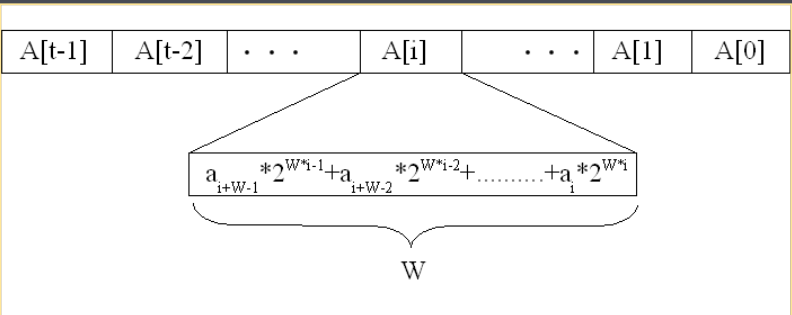
\includegraphics[width=0.8\textwidth]{figures/fig01-arrays-native-size}
    \centering
    \caption{Manuel Koschuch, Efficient Security for Mobile Communications Utilizing Elliptic Curves}
\end{figure}

\paragraph{Vorteile}

\begin{itemize}
    \item Die Langzahloperationen können auf Operationen auf nativer Wordgröße heruntergebrochen werden.
    \item Der zusätzliche Speicherbedarf ist maximal so groß wie ein natives Wort.
    \item Zugriff ist einfach und schnell.
    \item Vergleich von Langzahlen ist schnell und einfach.
    \item Verwendung von Langzahlen ist schnell und einfach.
\end{itemize}

\paragraph{Nachteile}

Operationen für diese Repräsentation sind nur bedingt parallelisierbar, es braucht hier eine carry-propagation.

%%% subsection %%%
\subsection{Arrays kleiner als die native Größe}

Sei wieder $W$ die native Wortgröße eines Prozessors und $x$ eine Zahl, deren Binärdarstellung $n$ bit benötigt. Jetzt verwenden wir das Array $A$, das 
$u = \lceil n/(W-k) \rceil$ Integers enthält, wobei $k$ ein für das entstehende Carry veranschlagter Speicher im Buffer ist.

\paragraph{Vorteile}

Hier haben wir ähnliche Vorteile wie bei Arrays in nativer Größe, zusätzlich haben wir Parallelisierbarkeit, weil zwei Worte addiert werden können, ohne dass carry-propagation 
notwendig wird.

\paragraph{Nachteile}

\begin{itemize}
    \item Potentiell höherer Speicherbedarf, da pro Wort $k$ Bit für carry frei bleiben
    \item Am Ende einer Rechnung muss carry sehr wohl propagiert werden (vgl. carry-save adders)
    \item Komplexere Behandlung der Elemente bei Rechnungen nötig, Konversion zu Beginn und am Ende einer Berechnung
\end{itemize}

%%% subsection %%%
\subsection{Exkurs: Basisoperationen}

Seien $b, k \in \mathbb{N}$. Für jedes Stellensystem zur Basis $b$ gilt:

\paragraph{Multiplikation}

Eine Multiplikation mit dem Faktor $b^k$ entspricht einem Linksshift um $k$ Stellen. Beispiel:

\begin{align*}
    & 145 \cdot 10^2 = 14500 \\
    & 1101 \cdot 2^3 = 1101000
\end{align*}

\paragraph{Integer-Division}

Eine Integer-Division durch den Divisor $b^k$ entspricht einem Rechtshift um $k$ Stellen. Beispiel:

\begin{align*}
    & 7654 / 10^3 = 7 \\
    & 1110011101 / 2^5 = 11100
\end{align*}

\paragraph{Niederwertigste Stellen extrahieren}

Eine Modulo Operation mit Modul $b^k$ entspricht dem extrahieren der $k$ niederwertigsten Stellen. Beispiel:

\begin{align*}
    & 65432 \mod 10^3 = 432 \\
    & 111000101 \mod 2^4 = 0101
\end{align*}

\paragraph{Casting out nines}

Eine Modulo Operation mit Modul $b^k - 1$ entspricht dem teiler einer Zahl in $k$-stellige Blöcke, die dann aufsummiert werden. Beispiel:

$$34215 \mod (10^2 - 1) = 34215 \mod 99 = 3 + 42 + 15 = 60$$

%%% subsection %%%
\subsection{Modulo Reduktion}

Eine Moduloreduktion ist die Berechnung des kleinsten Repräsentanten einer Restklasse. Beispiel: die Zahl $17 \mod 5$ wird zu 2 reduziert.

\paragraph{Kriterien für den Einsatz}

Wie können wir feststellen, wann eine Moduloreduktion überhaupt notwendig ist? Grundsätzlich kann immer mit nichtreduzierten Zwischenergebnissen gerechnet werden. In der 
Praxis ist es aber sinnvoll, eine Reduktion anzuwenden, wenn das Zwischenergebnis mehr als 1 bit länger als der Modulus ist. Diese Bedingung ist über ein logisches Und 
vom MSW (most significant word) des Zwischenergebnisses und einer Bitmaske abhängig vom Modul einfach feststellbar.

\paragraph{Kosten von Langzahldivisionen}

Divisionen von Wörtern sind teure Operationen auf Computern. Langzahldivisionen sind sogar noch teurer, wie können wir den Aufwand verringern?  

Hierfür gibt es Berechnungen von Divisionsresten ohne (tatsächliche) Divisionen, nämlich 

\begin{itemize}
    \item Barrett Reduktion 
    \item Montgomery Multiplikation
\end{itemize}

\paragraph{Barrett Reduktion} 

Die Rechnung $(a\cdot b) / n$ wird berechnet als 

$$\frac{a\cdot b}{b^{2k-t}} \cdot \frac{b^{2k}}{n} \cdot \frac{1}{b^t},$$

wobei $b$ die Basis der Zahlendarstellung (in Digitalsystemen also 2) ist.

\paragraph{Montgomery Multiplikation}

Wenn $R$ eine Zweierpotenz ist und es ein $n'$ gibt, sodass $R \cdot R^{-1} - n\cdot n' = 1$, dann wird $a \cdot b \cdot R^{-1} \mod n$ berechnet mittels 

$$\frac{a\cdot b + (a \cdot b \cdot n'\mod R \cdot n)}{R}.$$

Hierfür benötigt es eine Hin- und Rücktransformation.

Diese Ansätze sind nur bei mehreren modularen Multiplikationen hintereinander sinnvoll, ansonsten ist der Transformationsoverhead zu groß.

\paragraph{Grundidee an Montgomery (todo)}

Ein $k$-faches von $n$ zum Produkt addieren, so dass die letzten $i$ Stellen 0 werden, und sich damit die
Division auf ein reines Shift beschränkt.  

Wie bestimmt sich $k$? \newline
Für die letzte Stelle $c$ muss (im Dezimalsystem) gelten: 

\begin{align*}
&c + k\cdot n = 0 \mod 10  \\
 &\Rightarrow c = -k \cdot n \mod 10 \\
 &\Rightarrow c \cdot -n^{-1} = k \mod 10
\end{align*}

Für die folgenden Stellen gilt analoges, nur mit entsprechendem Offset um $10^i$.  


De facto also:
Das Produkt mit dem negativen Inversen des Moduls multiplizieren (was ja gerade $n'$ ist), das ganze
modulo $R$ rechnen (was ja die neue Basis darstellt und sich auf ein Bitmaskieren der letzten Bits
beschränkt, wenn $R$ eine Zweierpotenz ist), mit dem Modulus multiplizieren und zum Produkt
addieren. Damit sind garantiert die letzten Bits 0 und können durch die Division einfach rausgeshiftet
werden.


\paragraph{Montgomery Beispiel (todo)}

Ein Beispiel im Dezimalsystem: Seien $a = 29, b = 48, n = 97$ und $R = 100$.

\textit{Hintransformation}:

\begin{align*}
    a' = a \cdot R \mod n = 29 \cdot 100 \mod 97 = 2900 \mod 97 = 87 \\
    b' = b \cdot R \mod n = 48 \cdot 100 \mod 97 = 4800 \mod 97 = 47
\end{align*}

\textit{Multiplikation}

Es gilt $a' \cdot b' = 87 \cdot 47 = 4089$. Jetzt versuchen wir die letzte und vorletzte Stelle zu 0 zu machen:

\begin{align*}
    4089 + 3\cdot n = 408\textbf{9} + 3 \cdot 97 = 408\textbf{9} \cdot 29\textbf{1} = 4380 \\
    43\textbf{8}0 + 60 \cdot n = 43\textbf{8}0 + 60 \cdot 97 = 43\textbf{8}0 + 85\textbf{2}0 = 10200
\end{align*}

Jetzt dividieren wir durch $R = 100$: $10200 / 100 = 102$.

\textit{Rücktransformation}

Wir berechnen 

$$102 \cdot R^{-1} \mod n = 102 \cdot 100^{-1} \mod 97 = 102 \cdot 65 \mod 97 = 34.$$

In der Gegenprobe haben wir $a \cdot b \mod n = 29 \cdot 48 \mod 97 = 34$.

Für die Abschätzung von Montgomery haben wir das 

\begin{lemma}
    Seien $a, b, n \in \mathbb{N}$, dann gilt 
    \begin{equation}
        \frac{a\cdot b + (a\cdot b\cdot n' \mod R) \cdot n}{R} < 2n.
    \end{equation}
\end{lemma}

\begin{proof} (Skizze):
    Wir wissen $a, b < n$ und $R > n$. Daher gilt $a\cdot b < n^2$. Weiters gilt immer $a\cdot b \cdot n' \mod R < R$. Deswegen gilt 

    $$\frac{a\cdot b + (a\cdot b\cdot n' \mod R) \cdot n}{R} < \frac{n^2 + R \cdot n}{R} = \frac{n^2}{R} + \frac{R\cdot n}{R} < n\cdot 1 + n = 2n.$$
\end{proof}

\paragraph{Mongomery Pseudocode (todo)}

Eine komplette Montgomery Multiplikation ist daher:

\begin{verbatim}
Input: a, b
Output: c = a*b mod n

t = a * b
c = t + (t*n' mod R)*n //mit R*R' - n*n' = 1
c = c/R
if (c > n)
    c = c - n
return c
\end{verbatim}

\begin{centering}
Monty(a,b) = a*b*R-1 mod n \\
Monty(a',b) = a*b mod n \\
Monty(a',b') = a'*b' mod n \\
Monty(a',1) = a mod n \\
Monty(a,R*R) = a' mod n 
\end{centering}

\section{Exponentiation}

Exponentiation ist eine häufige Operation, gerade bei RSA. Dabei hat der private Exponent häufig auch mindestens 1024 bits. 

\subsection{Square-and-Multiply}

Square-and-Multiply is die formalisierte Variante der ``Methode der wiederholten Quadrate''. Für jedes bit im Exponenten wird quadriert, wenn die bits 1 sind, dann 
auch multipliziert.

\begin{verbatim}
    Berechne m = c^d 

    m = 1
    for jedes Bit i in d, beginnend bei MSB, do 
        m = m*m 
        if (i = 1) then
            m = m \cdot c
    end 
    return m
\end{verbatim}

\paragraph{Beispiel} Berechnen von $x^12$ mittels Square-and-Multiply, dafür betrachten wir die Binärdarstellung $12 = b1100$:

\begin{verbatim}
    m = 1

    # i = 1, erstes bit, beginnend beim größten
    m = m * m = 1
    m = m * x = x

    # i = 1, zweites bit
    m = m * m = x^2
    m = m * x = x^3

    # i = 0, drittes bit
    m = m * m = x^6

    # i = 0, viertes bit
    m = m * m = x^12
\end{verbatim}

Hier fällt auf: je mehr \verb|1|er in der Binärdarstellung der Exponenten, desto größer ist unser Rechenaufwand.


\paragraph{Beispiel} Wir berechnen eine RSA Verschlüsselung mit $m = 7, p = 5$ und $q = 11$.

Wir haben $\varphi = 40$ und wählen $e = 3$, dann gilt $d = 27$ und $c = m^e \mod (p\cdot q) = 7^3 \mod 55 = 13$. Mittels Square-and-Multiply berechnen wir $m = c^d = 7$:

\begin{verbatim}
    27 = b11011

    m = 1

    # i = 1
    m = m * m = 1
    m = m * c = 13

    # i = 1 
    m = m * m = 13 * 13 mod 55 = 4
    m = m * c = 4 * 13 mod 55 = 52

    # i = 0
    m = m * m = 52 * 52 mod 55 = 9

    # i = 1
    m = m * m = 9 * 9 mod 55 = 26
    m = m * c = 26 * 13 mod 55 = 8 

    # i = 1 
    m = m * m = 8 * 8 mod 55 = 9
    m = m * c = 9 * 13 mod 55 = 7
\end{verbatim}

\subsection{NAF - Non-adjacent Form}

Im Durchschnitt braucht es für die Berechnung einer Exponentiation mit einem $n$-bit Exponenten:

\begin{itemize}
    \item $n/2$ Multiplikationen und
    \item $n$ Quadrierungen.
\end{itemize}

Unter Verwendung einer vorzeichenbehafteten Darstellung des Exponenten (mit $-1, 0$ und $1$) kann die Anzahl der Multiplikationen auf $n/3$ reduziert werden. In diesem Fall
wird die NAF de Exponenten berechnet.

\paragraph{Eigenschaften}

\begin{itemize}
    \item Sie ist eindeutig
    \item Sie hat die wenigsten Elemente ungleich 0 aller vorzeichenbehafteten Darstellungen
    \item Sie ist maximal $n+1$ bit lang 
    \item Es folgen niemals zwei Elemente ungleich 0 aufeinander 
    \item Sie hat durchschnittlich n/3 Elemente ungleich 0
\end{itemize}

Die Exponentiation ist ähnlich zu Square-and-Multiply, es wird nur vor der Berechnung die Inverse der Basis berechnet und in den Fällen, wo das Bit -1 ist, mit diesem 
Inversen statt mit der Basis multipliziert.

\paragraph{Beispiel} 

Wir berechnen die NAF von 12. Wir wissen $12 = b1100$, ihre NAF ist $10-100$, weil $12 = 2^4 - 2^2 = 16 - 4$.

\paragraph{Beispiel}

Wir berechnen die NAF von 7. Wir wissen $7 = 111$, die NAF ist $100-1$, weil $7 = 2^3 - 2^0 = 8 - 1$. Die Rechnung $x^7$ mittels NAF:

\begin{verbatim}
7 = 100-1 (NAF)

m = 1

# i = 1
m = m * m = 1
m = m * x = x

# i = 0
m = m * m = x^2 

# i = 0
m = m * m = x^4

# i = -1
m = m * m = x^8
m = m * x^{-1} = x^7
\end{verbatim}

\paragraph{Private Key bei RSA}

Privater Schlüssel d bei RSA üblicherweise signifikant länger als öffentlicher (1.024 Bits vs. 16 Bits). Problem: Entschlüsselung und Signaturgenerierung teuer. \\

Lösung: mittels CRT (Chinesicher Restsatz). Statt nur $d$ zu speichern, werden $p$, $q$, $dP$, $dQ$ und $qInv$ einmalig berechnet und gespeichert. Hierbei ist:

\begin{align*}
dP &= d \mod (p-1) \\
dQ &= d \mod (q-1) \\
qInv &= q^{-1} \mod p
\end{align*}

Die Entschlüsselung wird nicht als $m = c^d \mod n$ berechnet, sondern 

\begin{align*}
    m_1 &= c^{dP} \mod p \\
    m_2 &= c^{dQ} \mod q \\
    h &= qInv \cdot (m_1 - m_2) \mod p \\
    m &= m_2 + h\cdot q
\end{align*}

Dadurch sind die Exponenten statt 1024 nur noch ca 512 Bit lang.

\begin{verbatim}
    Private-Key: (4096 bit, 2 primes)

    modulus: //n (4.096 Bit)
    00:[…]:5a:ac:58:ff:66:e7

    publicExponent: //e (17 Bit) 
    65537 (0x10001)
    
    privateExponent: //d (4.096 Bit)
    00:a0:4d:a3:d7:f5:[…]:36:96:67:e5:c1

    prime1: //p (2.048 Bit)
    00:ed:22:[…]64:2c:07

    prime2: //q (2.048 Bit)
    00:d9:3f:[…]41:f6:21

    exponent1: //dP (2.048 Bit)
    00:cf:f1:[…]7f:be:ef

    exponent2: //dQ (2.048 Bit)
    58:f6:5d:[…]3d:c8:a1

    coefficient: //qInv (2.048 Bit)
    00:e4:01:[…]76:dd:61:b8
\end{verbatim}
\chapter{Symmetrische Kryptographie}

Bei symmetrischer Kryptographie verwenden Sender und Empfänger denselben Schlüssel, das heißt die Ver- und Entschlüsselung passieren symmetrisch.
Bei Verschlüsselung gibt es zwei Arten:

\paragraph{Blockcipher}\index{Blockchipher} Die Daten werden in Blöcke fixer Größe aufgeteilt und verschlüsselt. Das ist sinnvoll, wenn es keine zeitliche Komponente bei 
den Daten gibt, 
und sie zum Zeitpunkt der Verschlüsselung bereits vollständig vorhanden sind. 

\paragraph{Streamcipher}\index{Streamchipher} Die Daten werden verschlüsselt, sobald sie zu Verfügung stehen, und werden dann laufend mit dem 
Schlüsselstrom\index{Schlüsselstrom}\index{Keystream} verknüpt. 
Das erfordert Synchronisation zwischen Sender und Empfänger. Dieser Verschlüsselungsmodus ist für zeitkritische Anwendungen geeignet, bei denen man nicht warten kann, bis 
ein kompletter Block an Daten vorhanden ist.

Bei beiden Varianten ist die wichtigste Voraussetzung, den verwendeten Schlüssel sicher zu übertragen.

\section{Blockchipher}

\begin{definition}[Blockcipher]\index{Blockchipher}
Ein Blockcipher mit einer Blocklänge von $n$ Bit ist eine invertierbare, üblicherweise deterministische Abbildung.

Sei $V_n = \{0, 1\}^n$ die Menge aller $n$ Bit Vektoren und $\mathcal{K} = \{0, 1\}^k$ die Menge aller $k$ Bit Vektoren, dann sind

$$E: V_n \times \mathcal{K} \to V_n \text{ und } D: V_n \times \mathcal{K} \to V_n$$

mit $E(m, \kappa) = c$ für ein beliebiges $m \in V_n, \kappa \in \mathcal{K}$ und $D(c, \kappa) = m$ ein Blockcipher.
\end{definition}

Wir verwenden die Notation $E_K(p) = E(p, K)$ für die Verschlüsselung mit dem fixen Schlüssel $K \in \mathcal{K}$ und analog $D_K(C)$ für die Entschlüsselung. Dann gilt 
für alle $P \in V_n$, dass $D_K(E_K(P)) = P$.

Die Sicherheit, aber auch die Komplexität wird durch die Blocklänge beeinflusst, hier muss ein Tradeoff gemacht werden. Es gilt es die Blocklänge unter Berücksichtigung 
der sicherheitstechnischen und performanten Anforderungen zu wählen. \\

Die Auswahlkriterien für Blockcipher sind:

\begin{itemize}
    \item Geschätztes Sicherheitslevel: Je bekannter und erforschter ein Cipher ist, als desto sicherer wird er angesehen
    \item Schlüsselgröße: Je höher die Entropie der Schlüsselt, desto höher ist die Sicherheit. Mit der Entropie steigt aber auch der Verarbeitungsaufwand.
    \item Durchsatz: Der Durchsatz eines Ciphers ist abhängig von seiner Komplexität.
    \item Blockgröße: Je größer die Blockgröße, desto höher die Sicherheit, aber auch die Komplexität.
    \item Komplexität der kryptographischen Abbildung: Sie beeinflusst die Größe sowohl einer Software- als auch einer Hardwareimplementierung.
    \item Datenexpansion: Gewisse Anwendungen erfordern, dass Daten vor und nach der Verschlüsselung dieselbe Größe haben.
    \item Fehlerfortpflanzung: Ein fehlerhafter Ciphertext hat Auswirkungen auf Klartext, die konkrete Auswirkung unterscheidet sich je nach Betriebsmodus und Cipher.
\end{itemize}

\subsection{ECB (Electronic Codebook Mode)}\index{Blockcipher Modi!ECB}\index{ECB}

Die Verschlüsselung von Plaintext Block $p_i$ ist

\begin{align*}
    c_i = E_K(p_i) \\
    p_i = D_K(c_i)
\end{align*}

Die Vorteile des ECB sind: 

\begin{itemize}
    \item Wahlfreier Zugriff
    \item Fehler in Ciphertext beeinflusst nur aktuellen Block
    \item Wenn nur Nachrichten von bis zu einem Block übertragen werden, sicher und effizient
\end{itemize}

Die Nachteile sind:

\begin{itemize}
    \item Muster in Klartext im Ciphertext sichtbar
    \item Selber Klartext ergibt bei selbem Schlüssel immer selben Ciphertext
    \item Block Replay Attacken: beliebige Ciphertextblöcke können entfernt, eingefügt oder ersetzt werden
\end{itemize}


\subsection{CBC (Cipher Block Chaining)}\index{Blockcipher Modi!CBC}\index{CBC}

Die Verschlüsselung von Plaintext Block $p_i$ ist

\begin{align*}
    c_i = E_K(p_i \oplus c_{i-1}) \\
    p_i = c_{i-1} \oplus D_K(c_i)
\end{align*}

Die Vorteile des CBC sind: 

\begin{itemize}
    \item Gleiche Klartextblöcke ergeben nur dann gleiche Ciphertextblöcke, wenn vorhergehende Klartextblöcke identisch sind
    \item Kein Block Replay mehr möglich
    \item Auf Block Ebene selbstheilend
\end{itemize}

Die Nachteile sind:

\begin{itemize}
    \item Ent- und Verschlüsselung können nicht mehr wahlfrei erfolgen
    \item Vor allem am Beginn oft gleiche Klartextblöcke, Lösung: zufälliger IV, braucht nicht geheim gehalten zu werden
    \item Ein 1-Bit Fehler in Cipherblock $c_i$ bewirkt einen völlig fehlerhaften Klartextblock $p_i$ und einen 1-Bit Fehler in $p_{i+1}$ (``Error Extension'')
    \item Einfügen beliebiger Blöcke am Ende bzw. gezielte Manipulation von Block $p_{i+1}$ möglich
\end{itemize}

\subsection{PCBC (Propagating Cipher Block Chaining)}\index{Blockcipher Modi!PCBC}\index{PCBC}

Die Verschlüsselung von Plaintext Block $p_i$ ist

\begin{align*}
    c_i = E_K(p_i \oplus c_{i-1} \oplus p_{i-1}) \\
    p_i = c_{i-1} \oplus p_{i-1} \oplus D_K(c_i)
\end{align*}

Die Vorteile des PCBC sind: 

\begin{itemize}
    \item Grundsätzlich gleiche Eigenschaften wie CBC
    \item Zusätzlich: Fehler im Ciphertext bewirkt Fehler in allen folgenden Blöcken
    \item Verwendet in Kerberos 4 zum Error-checking: wenn der letzte Block nicht dem erwarteten Wert entspricht, ist ein Fehler aufgetreten.
\end{itemize}

Die Nachteile sind:

\begin{itemize}
    \item Grundsätzlich gleiche Eigenschaften wie CBC
    \item Vertauschen zweier Ciphertext Blöcke führt zu teilweiser falscher Entschlüsselung, wegen XOR fällt Fehler aber beim nächsten Block wieder heraus
\end{itemize}

\paragraph{Beispiel} Vertauschen zweier Blöcke:

Wir berechnen den Ciphertext von der Nachricht $P = (P_1, P_2, P_3, P_4, P_5)$ und Initialisierungsvektor $IV$:

\begin{align*}
    C_1 &= E_K(P_1 \oplus IV) \\
    C_2 &= E_K(P_2 \oplus C_1 \oplus P_1) \\
    C_3 &= E_K(P_3 \oplus C_2 \oplus P_2) \\
    C_4 &= E_K(P_4 \oplus C_3 \oplus P_3) \\
    C_5 &= E_K(P_5 \oplus C_4 \oplus P_4) \\
\end{align*}

Und erhalten $C = (IV, C_1, C_2, C_3, C_4, C_5)$. Jetzt manipuliert ein Angreifer den Ciphertext und wir entschlüsseln statt $C$ den Text 
$C'= (IV, C_1, C_\mathbf{3}, C_\mathbf{2}, C_4, C_5)$. Wir entschlüsseln:

\begin{align*}
    P_1 &= D_K(C_1) \oplus IV = (P_1 \oplus IV) \oplus IV = P_1 \\
    P'_2 &= D_K(C_3) \oplus P_1 \oplus C_1 = (P_3 \oplus C_2 \oplus P_2) \oplus P_1 \oplus C_1 \\
    P'_3 &= D_K(C_2) \oplus P'_2 \oplus C_3 = (P_2 \oplus C_1 \oplus P_1) \oplus P'_2 \oplus C_3 \\
         &= (P_2 \oplus C_1 \oplus P_1) \oplus (P_3 \oplus C_2 \oplus P_2 \oplus P_1 \oplus C_1) \oplus C_3 = P_3 \oplus C_2 \oplus C_3\\
    P_4 &= D_K(C_4) \oplus P'_3 \oplus C_2 = (P_4 \oplus C_3 \oplus P_3) \oplus (P_3 \oplus C_2 \oplus C_3) \oplus C_2 = P_4\\
    P_5 &= D_K(C_5) \oplus P_4 \oplus C_4 = (P_5 \oplus C_4 \oplus P_4) \oplus P_4 \oplus C_4 = P_5
\end{align*}

Das heißt, aus dem Cipher $C' = (IV, C_1, C_3, C_2, C_4, C_5)$ ist der Plaintext 
$P' = (P_1, P_3 \oplus C_2 \oplus P_2 \oplus P_1 \oplus C_1,  P_3 \oplus C_2 \oplus C_3, P_4, P_5)$ entstanden und nur die vertauschten Blöcke sind fehlerhaft.

\subsection{XTS (oder XEX-TCB-CTS)}\index{Blockcipher Modi!XTS}\index{XTS}\index{XEX-TCB-CTS}

Für das Xor-Encrypt-Xor-based Tweaked CodeBook Mode with CipherText Stealing brauchen wir einen geteilten Schlüssel $K = K_1 || K_2$, ein Tweak $i$ mit einem dazugehörigen 
$j$ (z.B. ist $i$ die Blocknummer auf der Harddisk unf $j$ der entsprechende Sektor) und ein $\alpha$, das ein primitives Element in $GF(2^{128})$ ist. 
Es gilt für die Ver- und Entschlüsselung:

\begin{align*}
    c_j &= E_{K_1}\left(p_i \oplus (E_{K_2}(j) \oplus \alpha^i)\right) \oplus \left(E_{K_2}(j) \oplus \alpha^i\right) \\
    p_j &= D_{K_1}\left(c_i \oplus (E_{K_2}(j) \oplus \alpha^i)\right) \oplus \left(E_{K_2}(j) \oplus \alpha^i\right)
\end{align*}

\begin{figure}[h]
    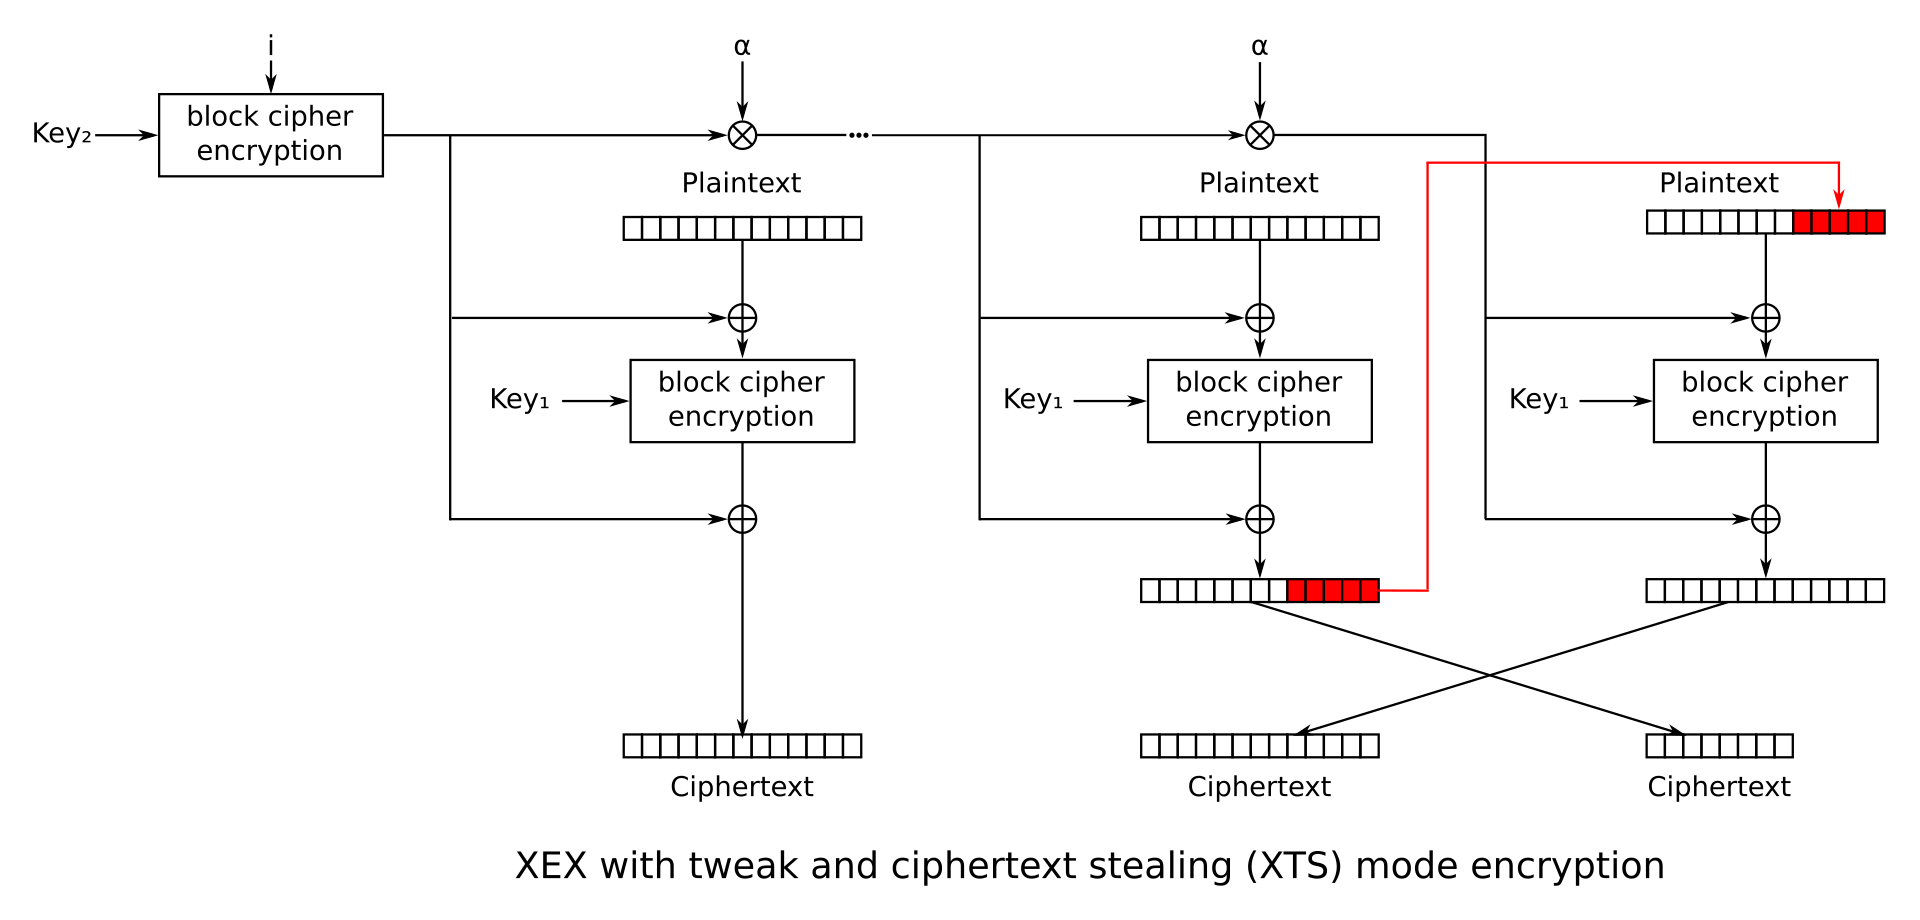
\includegraphics[width=0.8\textwidth]{figures/fig02-XTS_mode_encryption}
    \centering
    \caption{Aorimn, \href{https://creativecommons.org/licenses/by-sa/4.0}{CC BY-SA 4.0}, via Wikimedia Commons}
\end{figure}

Die Vorteile sind 

\begin{itemize}
    \item deal für Datenverschlüsselung an Endpunkten (Festplattenverschlüsselung)
    \item Ciphertext ist gleich lang wie Klartext
\end{itemize}

Die Nachteile sind

\begin{itemize}
    \item Schlüsselteilung ($K_1$ und $K_2$) potentiell unnötig und verkompliziert Vorgang
    \item Kein Authentication Tag
\end{itemize}

\subsection{Exkurs: CTS (Cipher Text Stealing)}\index{CTS}\index{Cipher Text Stealing}

Grundproblem: wenn der letzte Klartextblock kleiner ist als die Blockgröße, muss dieser aufgefüllt werden. Damit wird aber der Ciphertext größer als der Klartext. \\

Lösung: Sei $b$ die Blockgröße und $P = (P_1, \ldots, P_n)$ der Klartext.

\begin{enumerate}
    \item der letzte komplette Klartextblock $P_{-1}$ wird zu (Achtung) $C_\mathbf{n}$ verschlüsselt 
    \item der letzte Klartextblock $P_n$ wird mit den letzten $l$ Bits von $C_n$ aufgefüllt
    \item der neue letzter Block wird verschlüsselt, ergibt $C_\mathbf{n-1}$
    \item Die ersten $b-l$ Bits von $C_n$ ergeben den neuen letzten Block
\end{enumerate}

% width=0.8\textwidth
\begin{figure}[h]
    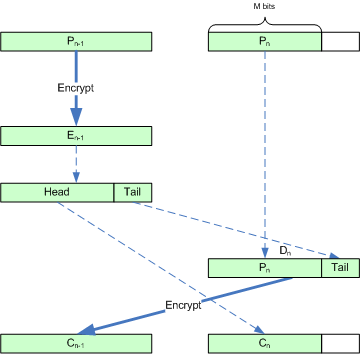
\includegraphics[width=0.4\textwidth]{figures/fig03-CTS_ECB_Encryption}
    \centering
    \caption{Yaronf, \href{https://creativecommons.org/licenses/by-sa/4.0}{CC BY-SA 4.0}, via Wikimedia Commons}
\end{figure}

\subsection{Auswahl des Blockcipher Modus}\index{Blockcipher Modi}

Folgende Empfehlungen gibt es für die Auswahl der Blockcipher Modi:

\begin{center}
    \begin{tabular}{ ll } 
        \hline
        Anwendungsfall & Modus \\ 
        \hline
        Kurze, zufällige Daten & (ECB) GCM \\
        Daten in der Übertragung & GCM \\
        Gespeicherte, große Daten & XTS \\
        \hline
    \end{tabular}
\end{center}

Andere Modi sind, wenn möglich, zu vermeiden.

\subsection{DES (Data Encryption Standard)}\index{DES}

Das NBS, der Vorläufer des heutigen NIST, beschloss 1972 einen standardisierten Verschlüsselungsalgorithmus zu entwickeln. Die Anforderungen daran waren:

\begin{itemize}
    \item Hohes Sicherheitslevel
    \item Leicht zu verstehen und lückenlos spezifiziert
    \item Sicherheit liegt im Schlüssel, nicht im Algorithmus
    \item Mit vertretbarem wirtschaftlichen Aufwand in elektronische Geräte integrierbar
    \item ``Frei'' verfügbar
    \item Anpassbar
    \item Effizient
    \item Validierbar
    \item Exportierbar
\end{itemize}

Beim ersten Aufruf gab es keine (brauchbaren) Einsendungen, beim zweiten (1974) dann eine von IBM, Lucifer. Dieser wurde mit Hilfe der NSA evaluiert, verändert und 
1975 veröffentlicht, ab 1976 Standard. DES wurde weitflächig übernommen, auch von Banken, Einzelhandel, Telekommunikation, etc.

Laut heutiger Aussage war die Veröffentlichung der ``größter Fehler der NSA'' - sie war der Meinung, es ginge bei DES nur um Hardwareimplementierungen.
Bis 1994 nur Hardware zertifiziert, keine Software. Ab 1983 wurde der Standard alle 5 Jahre reviewt:

\begin{itemize}
    \item 1983 problemlos
    \item 1988 Einspruch der NSA, ``likely to be broken''
    \begin{itemize}
        \item Als Alternative COMSEC
        \item Große Gegenwehr, Vorschlag abgelehnt
        \item NSA stimmte dann doch Rezertifizierung zu, mit Bedingung ``nie wieder''
    \end{itemize}
    \item 1993 wieder zertifiziert
    \item 1999 ebenso, mit Empfehlung, 3DES zu verwenden
    \item 2004 Standard (FIPS 46-3) zurückgezogen
\end{itemize}

DES ist ein symmetrischer Blockcipher mit Blockgröße 64 Bit. Die Schlüsselgröße ist 64 Bit, aber effektiv nur 56, da jedes 8.Bit ein Prüfbit ist. \\

Die Grundprinzipien ist Konfusion und Diffusion: Konfusion \index{Konfusion}\index{Blockcipher!Konfusion} heißt, die Beziehung zwischen Klartext, Schlüssel und Ciphertext soll so komplex wie möglich 
sein.
Diffusion \index{Diffusion}\index{Blockcipher!Diffusion} heißt, der Ciphertext hängt von so vielen Klartext Bits ab wie nur möglich.

DES wird mittels Permutationen und Substitutionen realisiert, die 16 Mal (als ``Runden'') wiederholt werden. Diese Struktur eignet sich sehr gut für 
Hardwareimplementierungen.

\begin{enumerate}
    \item Der 64-Bit Input wird initial permutiert.
    \item Das Ergebnis vom letzten Schritt wird in zwei Hälften $L_0$ und $R_0$ gespalten
    \item In einer Schleife wird 16 Mal ein Folgeergebnis berechnet: 
    \begin{enumerate}
        \item $L_i = R_{i-1}$
        \item $R_i = L_{i-1} \oplus f(R_{i-1}, K_i)$
    \end{enumerate}
    \item Für das Endergebnis werden beide Hälften zusammengefügt und final permutiert, das Ergebnis hat wie der Input 64 Bit.
\end{enumerate}

Die Entschlüsselung erfolgt bei DES völlig symmetrisch zur Verschlüsselung, einzig die Rundenkeys müssen in umgekehrter Reihenfolge erzeugt und verwendet werden.

Die zertifizierten Modi von DES sind ECB, CBC, OFB (Output Feedback Mode) und CFB (Cipher feedback). Implementierungen: zwischen 700 Mbit/sec (Software, OpenSSL) und 
768.000.000.000 keys/sec (Hardware, crack.sh). Der DES wird heute nicht mehr weiterentwickelt.

Betrachten wir die einzelnen Schritte:

\paragraph{Initiale und finale Permutation}

Die finale Permutation ist invers zur initialen.
Diese Permutation haben keinen Einfluss auf die Sicherheit, sondern wurden eingeführt um das Einlesen der Bytes in Hardware zu erleichtern. Bei Softwareimplementierungen 
werden sie oft ausgelassen, weil sie dort schwer und mit vielen Bitoperationen implementiert werden müssten.

\begin{figure}[h]
    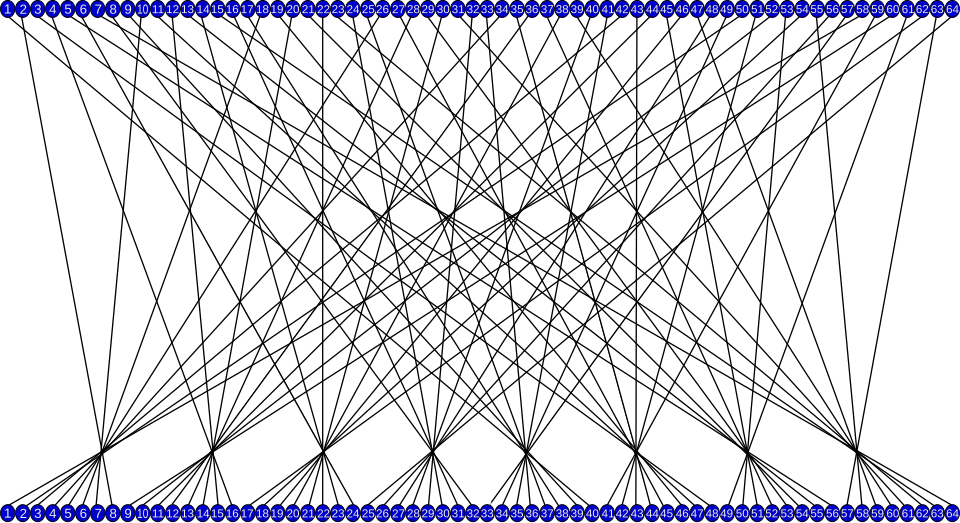
\includegraphics[width=0.8\textwidth]{figures/fig04-Permutation_initiale.png}
    \centering
    \caption{Initiale Permutation der 64 Bit, Quelle: Bourrichon, \href{https://creativecommons.org/licenses/by-sa/4.0}{CC BY-SA 4.0}, via Wikimedia Commons}
\end{figure}

\paragraph{Key Transformation mit Compression Permutation}

Bei der Key Transformation wird vom 64-Bit Key jedes 8. Bit verworfen. Die übrigen Bits werden in zwei Hälften zu je 28 Bit geteilt und in 16 Runden zirkulär nach links 
geshiftet. Dabei wird fast immer um 2 Bit geshiftet, außer in Runden 1, 2, 9 und 16, wo nur um 1 Bit geshiftet wird.

\begin{table}[h]
    \centering
        \begin{tabular}{|*{16}{c|}}
        \hline
        % Row 1 (cells 1-16)
        \cellcolor{red-1}1 & \cellcolor{red-1}2 & \cellcolor{red-1}3 & \cellcolor{red-1}4 & 
        \cellcolor{red-1}5 & \cellcolor{red-1}6 & \cellcolor{red-1}7 & \cellcolor{red-1}8 & 
        \cellcolor{yellow-1}9 & \cellcolor{yellow-1}10 & \cellcolor{yellow-1}11 & \cellcolor{yellow-1}12 & 
        \cellcolor{yellow-1}13 & \cellcolor{yellow-1}14 & \cellcolor{yellow-1}15 & \cellcolor{yellow-1}16 \\
        \hline
        % Row 2 (cells 17-32)
        \cellcolor{green-1}17 & \cellcolor{green-1}18 & \cellcolor{green-1}19 & \cellcolor{green-1}20 & 
        \cellcolor{green-1}21 & \cellcolor{green-1}22 & \cellcolor{green-1}23 & \cellcolor{green-1}24 & 
        \cellcolor{blue-1}25 & \cellcolor{blue-1}26 & \cellcolor{blue-1}27 & \cellcolor{blue-1}28 & 
        \cellcolor{blue-1}29 & \cellcolor{blue-1}30 & \cellcolor{blue-1}31 & \cellcolor{blue-1}32 \\
        \hline
        % Row 3 (cells 33-48)
        \cellcolor{orange-1}33 & \cellcolor{orange-1}34 & \cellcolor{orange-1}35 & \cellcolor{orange-1}36 & 
        \cellcolor{orange-1}37 & \cellcolor{orange-1}38 & \cellcolor{orange-1}39 & \cellcolor{orange-1}40 & 
        \cellcolor{purple-1}41 & \cellcolor{purple-1}42 & \cellcolor{purple-1}43 & \cellcolor{purple-1}44 & 
        \cellcolor{purple-1}45 & \cellcolor{purple-1}46 & \cellcolor{purple-1}47 & \cellcolor{purple-1}48 \\
        \hline
        % Row 4 (cells 49-64)
        \cellcolor{cyan-1}49 & \cellcolor{cyan-1}50 & \cellcolor{cyan-1}51 & \cellcolor{cyan-1}52 & 
        \cellcolor{cyan-1}53 & \cellcolor{cyan-1}54 & \cellcolor{cyan-1}55 & \cellcolor{cyan-1}56 & 
        \cellcolor{magenta-1}57 & \cellcolor{magenta-1}58 & \cellcolor{magenta-1}59 & \cellcolor{magenta-1}60 & 
        \cellcolor{magenta-1}61 & \cellcolor{magenta-1}62 & \cellcolor{magenta-1}63 & \cellcolor{magenta-1}64 \\
        \hline
        \end{tabular}
    \caption{Input Array für den Schlüssel mit 64 Bit}
\end{table}

\begin{table}[h]
    \centering
    \begin{minipage}[t]{0.45\textwidth}
        \begin{tabular}{|*{7}{c|}}
            \hline
            \cellcolor{magenta-1}57 & \cellcolor{cyan-1}49 & \cellcolor{purple-1}41 & \cellcolor{orange-1}33 & 
            \cellcolor{blue-1}25 & \cellcolor{green-1}17 & \cellcolor{yellow-1}9 \\

            \hline
            \cellcolor{red-1}1 & \cellcolor{magenta-1}58 & \cellcolor{cyan-1}50 & \cellcolor{purple-1}42 & 
            \cellcolor{orange-1}34 & \cellcolor{blue-1}26 & \cellcolor{green-1}18 \\

            \hline
            \cellcolor{yellow-1}10 & \cellcolor{red-1}2 & \cellcolor{magenta-1}59 & \cellcolor{cyan-1}51 & 
            \cellcolor{purple-1}43 & \cellcolor{orange-1}35 & \cellcolor{blue-1}27 \\

            \hline
            \cellcolor{green-1}19 & \cellcolor{yellow-1}11 & \cellcolor{red-1}3 & \cellcolor{magenta-1}60 & 
            \cellcolor{cyan-1}52 & \cellcolor{purple-1}44 & \cellcolor{orange-1}36  \\
            \hline
        \end{tabular}
    \end{minipage}
    \hfill
    \begin{minipage}[t]{0.45\textwidth}
        \begin{tabular}{|*{7}{c|}}
            \hline
            \cellcolor{magenta-1}63 & \cellcolor{cyan-1}55 & \cellcolor{purple-1}47 & \cellcolor{orange-1}39 & 
            \cellcolor{blue-1}31 & \cellcolor{green-1}23 & \cellcolor{yellow-1}15 \\

            \hline
            \cellcolor{red-1}7 & \cellcolor{magenta-1}62 & \cellcolor{cyan-1}54 & \cellcolor{purple-1}46 & 
            \cellcolor{orange-1}38 & \cellcolor{blue-1}30 & \cellcolor{green-1}22 \\

            \hline
            \cellcolor{yellow-1}14 & \cellcolor{red-1}6 & \cellcolor{magenta-1}61 & \cellcolor{cyan-1}53 & 
            \cellcolor{purple-1}45 & \cellcolor{orange-1}37 & \cellcolor{blue-1}29 \\

            \hline
            \cellcolor{green-1}21 & \cellcolor{yellow-1}13 & \cellcolor{red-1}5 & \cellcolor{blue-1}28 & 
            \cellcolor{green-1}20 & \cellcolor{yellow-1}12 & \cellcolor{red-1}4  \\
            \hline
        \end{tabular}
    \end{minipage}
    \caption{Output Arrays mit den Schlüsseln $K_1$ und $K_2$}
\end{table}

Nach dem Shiften werden aus den übrigen 56 Bits 48 ausgewählt und permutiert (``Compression Permutation''\index{Compression Permutation}):

\begin{table}[h]
    \centering
    \begin{tabular}{|*{14}{c|}}
        \hline
        % Row 1 
        \cellcolor{red-1}1 & \cellcolor{red-1}2 & \cellcolor{red-1}3 & \cellcolor{red-1}4 & 
        \cellcolor{red-1}5 & \cellcolor{red-1}6 & \cellcolor{red-1}7 & \cellcolor{red-1}8 & 
        \cellcolor{orange-1}9 & \cellcolor{orange-1}10 & \cellcolor{orange-1}11 & \cellcolor{orange-1}12 & 
        \cellcolor{orange-1}13 & \cellcolor{orange-1}14\\
        \hline
        % Row 2 
        \cellcolor{orange-1}15 & \cellcolor{orange-1}16 & 
        \cellcolor{yellow-1}17 & \cellcolor{yellow-1}18 & \cellcolor{yellow-1}19 & \cellcolor{yellow-1}20 & 
        \cellcolor{yellow-1}21 & \cellcolor{yellow-1}22 & \cellcolor{yellow-1}23 & \cellcolor{yellow-1}24 & 
        \cellcolor{green-1}25 & \cellcolor{green-1}26 & \cellcolor{green-1}27 & \cellcolor{green-1}28 \\
        \hline
        % Row 3 
        \cellcolor{green-1}29 & \cellcolor{green-1}30 & \cellcolor{green-1}31 & \cellcolor{green-1}32 &
        \cellcolor{cyan-1}33 & \cellcolor{cyan-1}34 & \cellcolor{cyan-1}35 & \cellcolor{cyan-1}36 & 
        \cellcolor{cyan-1}37 & \cellcolor{cyan-1}38 & \cellcolor{cyan-1}39 & \cellcolor{cyan-1}40 & 
        \cellcolor{blue-1}41 & \cellcolor{blue-1}42 \\
        \hline 
        % Row 4 
        \cellcolor{blue-1}43 & \cellcolor{blue-1}44 & 
        \cellcolor{blue-1}45 & \cellcolor{blue-1}46 & \cellcolor{blue-1}47 & \cellcolor{blue-1}48 &
        \cellcolor{purple-1}49 & \cellcolor{purple-1}50 & \cellcolor{purple-1}51 & \cellcolor{purple-1}52 & 
        \cellcolor{purple-1}53 & \cellcolor{purple-1}54 & \cellcolor{purple-1}55 & \cellcolor{purple-1}56 \\
        \hline
    \end{tabular}
    \caption{Input Array für mit 56 Bit}
\end{table}

\begin{table}[h]
    \centering
    \begin{tabular}{|*{12}{c|}}
        \hline
        % Row 1 
        \cellcolor{orange-1}14 & \cellcolor{yellow-1}17 & \cellcolor{orange-1}11 & \cellcolor{yellow-1}24 & 
        \cellcolor{red-1}1 & \cellcolor{red-1}5 & \cellcolor{red-1}3 & \cellcolor{green-1}28 &
        \cellcolor{orange-1}15 & \cellcolor{red-1}6 & \cellcolor{yellow-1}21 & \cellcolor{orange-1}10 \\
        \hline 
        
        % Row 2 
        \cellcolor{yellow-1}23 & \cellcolor{yellow-1}19 & \cellcolor{orange-1}12 & \cellcolor{red-1}4 & 
        \cellcolor{green-1}26 & \cellcolor{red-1}8 & \cellcolor{orange-1}16 & \cellcolor{red-1}7 & 
        \cellcolor{green-1}27 & \cellcolor{yellow-1}20 & \cellcolor{orange-1}13 & \cellcolor{red-1}2 \\
        \hline

        
        % Row 3  
        \cellcolor{blue-1}41 & \cellcolor{purple-1}52 & \cellcolor{green-1}31 & \cellcolor{cyan-1}37 & 
        \cellcolor{blue-1}47 & \cellcolor{purple-1}55 & \cellcolor{green-1}30 & \cellcolor{cyan-1}40 & 
        \cellcolor{purple-1}51 & \cellcolor{blue-1}45 & \cellcolor{cyan-1}33 & \cellcolor{blue-1}48 \\
        \hline

        % Row 4 
        \cellcolor{blue-1}44 & \cellcolor{purple-1}49 & \cellcolor{cyan-1}39 & \cellcolor{purple-1}56 &
        \cellcolor{cyan-1}34 & \cellcolor{purple-1}53 & \cellcolor{blue-1}46 & \cellcolor{blue-1}42 &
        \cellcolor{purple-1}50 & \cellcolor{cyan-1}36 & \cellcolor{green-1}29 & \cellcolor{green-1}32 \\
        \hline
    \end{tabular}
    \caption{Output Array nach ``Compression Permutation'' (48 bit)}
\end{table}

\begin{itemize}
    \item Weil jedes 8te Bit im Key ein Parity Bit ist, ist die faktische Länge des Keys statt 64 nur 56 Bit. 
    \item Für jede Runde muss ein anderer Schlüssel verwendet werden 
    \item Shiften ist schnell und billig in HW implementierbar 
    \item In keiner Runde wird der gesamte Schlüssel verwendet 
    \item Sicher gegen Related Key Analysis
\end{itemize}

\paragraph{Expansion Permutation}

In jeder Runde wird die Hälfte $R_i$ (32 Bit) mit dem 48 Bit Key xor-t werden. Dafür wird die Expansion Permutation \index{Expansion Permutation} verwendet. Hier gibt
es einen Lawinen Effekt (Avalanche Effect), wo möglichst viele Input Bits den Output beeinflussen (und umgekehrt). Das jeweils 1. und 4. Bit eines Blocks wird verdoppelt.

\begin{table}[h]
    \centering
    \begin{tabular}{|*{8}{c|}}
        \hline
        % Row 1 
        \cellcolor{red-1}1 & \cellcolor{red-1}2 & \cellcolor{red-1}3 & \cellcolor{red-1}4 & 
        \cellcolor{red-1}5 & \cellcolor{red-1}6 & \cellcolor{red-1}7 & \cellcolor{red-1}8 \\
        \hline 
        % Row 2 
        \cellcolor{orange-1}9 & \cellcolor{orange-1}10 & \cellcolor{orange-1}11 & \cellcolor{orange-1}12 & 
        \cellcolor{orange-1}13 & \cellcolor{orange-1}14 & \cellcolor{orange-1}15 & \cellcolor{orange-1}16 \\
        \hline 
        % Row 3
        \cellcolor{yellow-1}17 & \cellcolor{yellow-1}18 & \cellcolor{yellow-1}19 & \cellcolor{yellow-1}20 & 
        \cellcolor{yellow-1}21 & \cellcolor{yellow-1}22 & \cellcolor{yellow-1}23 & \cellcolor{yellow-1}24 \\
        \hline
        % Row 4 
        \cellcolor{green-1}25 & \cellcolor{green-1}26 & \cellcolor{green-1}27 & \cellcolor{green-1}28 &
        \cellcolor{green-1}29 & \cellcolor{green-1}30 & \cellcolor{green-1}31 & \cellcolor{green-1}32 \\
        \hline 
    \end{tabular}
    \caption{Input Array $R_i$ (32 Bit)}
\end{table}

\begin{table}[h]
    \centering
    \begin{tabular}{|*{12}{c|}}
        \hline
        % Row 1 
        \cellcolor{green-1}32 &
        \cellcolor{red-1}1 & \cellcolor{red-1}2 & \cellcolor{red-1}3 & \cellcolor{red-1}4 & 
        \cellcolor{red-1}5 & \cellcolor{red-1}6 & \cellcolor{red-1}7 & \cellcolor{red-1}8 & \cellcolor{orange-1}9\\
        \hline 
        % Row 2 
        \cellcolor{red-1}8 &
        \cellcolor{orange-1}9 & \cellcolor{orange-1}10 & \cellcolor{orange-1}11 & \cellcolor{orange-1}12 & 
        \cellcolor{orange-1}13 & \cellcolor{orange-1}14 & \cellcolor{orange-1}15 & \cellcolor{orange-1}16 & \cellcolor{yellow-1}17 \\
        \hline 
        % Row 3
        \cellcolor{orange-1}16 &
        \cellcolor{yellow-1}17 & \cellcolor{yellow-1}18 & \cellcolor{yellow-1}19 & \cellcolor{yellow-1}20 & 
        \cellcolor{yellow-1}21 & \cellcolor{yellow-1}22 & \cellcolor{yellow-1}23 & \cellcolor{yellow-1}24 & \cellcolor{green-1}25\\
        \hline
        % Row 4 
        \cellcolor{yellow-1}24 &
        \cellcolor{green-1}25 & \cellcolor{green-1}26 & \cellcolor{green-1}27 & \cellcolor{green-1}28 &
        \cellcolor{green-1}29 & \cellcolor{green-1}30 & \cellcolor{green-1}31 & \cellcolor{green-1}32 & \cellcolor{red-1}1\\
        \hline 
    \end{tabular}
    \caption{Zwischenergebnis Array für Expansion Permutation}
\end{table}

\begin{table}[h]
    \centering
    \begin{tabular}{|*{12}{c|}}
        \hline
        % Row 1 
        \cellcolor{orange-1}14 & \cellcolor{yellow-1}17 & \cellcolor{orange-1}11 & \cellcolor{yellow-1}24 & \cellcolor{red-1}1 & 
        \cellcolor{red-1}5 & \cellcolor{red-1}3 & \cellcolor{green-1}28 & \cellcolor{orange-1}15 & \cellcolor{red-1}6 & 
        \cellcolor{yellow-1}21 & \cellcolor{orange-1}10 \\
        \hline 
        % Row 2 
        \cellcolor{yellow-1}23 & \cellcolor{yellow-1}19 & \cellcolor{orange-1}12 & \cellcolor{red-1}4 & \cellcolor{green-1}26 & 
        \cellcolor{red-1}8 & \cellcolor{orange-1}16 & \cellcolor{red-1}7 & \cellcolor{green-1}27 & \cellcolor{yellow-1}20 & 
        \cellcolor{orange-1}13 & \cellcolor{red-1}2 \\
        \hline 
        % Row 3
        \cellcolor{blue-1}41 & \cellcolor{blue-1}52 & \cellcolor{green-1}31 & \cellcolor{blue-1}37 & \cellcolor{blue-1}47 & 
        \cellcolor{blue-1}55 & \cellcolor{green-1}30 & \cellcolor{blue-1}40 & \cellcolor{blue-1}51 & \cellcolor{blue-1}45 & 
        \cellcolor{blue-1}33 & \cellcolor{blue-1}48 \\
        \hline
        % Row 4 
        \cellcolor{blue-1}44 & \cellcolor{blue-1}49 & \cellcolor{blue-1}39 & \cellcolor{blue-1}56 & \cellcolor{blue-1}34 & 
        \cellcolor{blue-1}53 & \cellcolor{blue-1}46 & \cellcolor{blue-1}42 & \cellcolor{blue-1}50 & \cellcolor{blue-1}36 & 
        \cellcolor{green-1}29 & \cellcolor{green-1}32 \\
        \hline 
    \end{tabular}
    \caption{Output Array nach Expansion Permutation (sic)}
\end{table}

\begin{itemize}
    \item Der Datenblock muss auf Schlüsselgröße erweitert werden
    \item Durch Wiederholung einzelner Bits breitet sich Einfluss des Inputs aufden Output schneller aus (ein Inputbit beeinflusst 2 S-Box Lookups)
\end{itemize}

\paragraph{S-Boxen}

Der expandierte Block $R_i$ wird mit dem komprimierten Rundenschlüssel ver-xor-t. Der resultierende 48 Bit Block wird in 8 6er-Blöcke aufgeteilt. Jeder dieser 6 Bit 
Blöcke kommt in eine eigene S-Box.

Jede S-Box enthält 4 Zeilen zu je 16 Spalten und hat 4 Bit große Einträge.

\begin{itemize}
    \item Bits (1, 6) indizieren die Zeile (00, 01, 10, 11)
    \item Bits (2, 3, 4, 5) indizieren die Spalte (0000, 0001, \ldots, 1111)
    \item Beispiel: Der 6 Bit Input \verb|100111| wird auf den Eintrag in Zeile 4 (\verb|11|), Spalte 4 (\verb|0011|) gemapped
\end{itemize}

Aus den 48 (= $8 \cdot 6$) Bit Input wird über eine nicht-lineare Operation so ein 32 (= $8 \cdot 4$) Output generiert. Dieser Schritt ist besonders wichtig in DES.

Die Designkriterien für die S-Boxen (vgl. Don Coppersmith, The Data Encryption Standard (DES) and its strength against attacks) waren: 
\begin{itemize}
    \item Wegen HW und Technologie Beschränkungen (1974) waren nicht mehr als 6 Input- und 4 Output-Bits möglich 
    \item Kein Output Bit darf nahe einer linearen Funktion der Input Bits sein 
    \begin{itemize}
        \item Für jedes Output Bit und jeder Menge der 6 Input Bits ist das XOR dieser Inputs in ca. 50\% der Fälle gleich dem Output Bit
    \end{itemize}
    \item Jeder mögliche 4-Bit Output wird angenommen
    \item Wenn sich 2 Inputs um 1 Bit unterschieden, unterschiedet sich der Output um mindestens 2 Bit
    \item Wenn sich 2 Inputs nur in den beiden mittleren Bits unterscheiden, unterscheidet sich der Output in mindestens 2 Bit
    \item Wenn die ersten beiden Bits zweier Inputs anders, die letzten beiden gleich sind, dann ist der Output niemals ident
\end{itemize}

\paragraph{P-Boxen}

Nach der Substitution werden die 32 Bit noch einmal permutiert. Zum Abschluss werden die 32 Bit noch mit der linken Datenhälfte ver-xor-t. 
Danach werden $R_i$ und $L_i$ vertauscht. (todo: Tabelle einfügen)

Die Designkriterien der P-Boxen waren:

\begin{itemize}
    \item Die Output Bits von Runde $i$ (4 Bit) werden so verteilt, dass
    \begin{itemize}
        \item zwei der Bits in der Folgerunde zu den ``mittleren'' Bits einer S-Box werden. 
        \item zwei der Bits in der Folgerunde zu den ``Endbits'' werden. 
        \item sechs unterschiedliche S-Boxen dadurch beeinflusst werden.
    \end{itemize}
\end{itemize}

\paragraph{DES Runden}

\begin{figure}[h]
    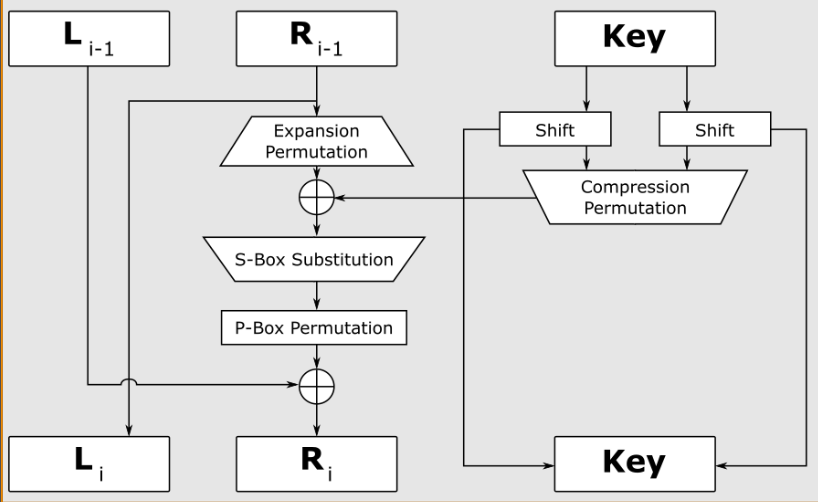
\includegraphics[width=0.8\textwidth]{figures/fig05-des-round.png}
    \centering
    \caption{Eine Runde in DES, Bruce Schneier, Applied Cryptography, 2nd Edition, Fig. 12.2}
\end{figure}


Nach 5 Runden ist jedes Outputbit eine Funktion jedes Input- und jedes Keybits.
Nach 8 Runden ist der Output quasi eine Zufallsfunktion -- aber durch differentielle Kryptoanalyse ((wieder)entdeckt 1990)
kann jede DES Implementierung innerhalb von 16 Runden gebrochen werden. 

\paragraph{Sicherheitsbetrachtungen div. Schlüssel}

Es gibt Weak Keys \index{Weak keys}, bei diesen besteht mindestens eine Hälfte (potentiell der gesamte Schlüssel) aus nur \verb|0| oder \verb|1|. Dadurch wird in jeder 
Runde derselbe Subkey erzeugt. Es gibt 4 verschiedene Weak Keys:

\begin{itemize}
    \item \verb|0x0101010101010101|
    \item \verb|0xFEFEFEFEFEFEFEFE|
    \item \verb|0xE0E0E0E0F1F1F1F1|
    \item \verb|0x1F1F1F1F0E0E0E0E|
\end{itemize}

Bei Semiweak Keys \index{Semiweak Keys} werden statt 16 unterschiedlicher Subkeys nur 2 erzeugt. Nachrichten die mit einem der Schlüsseln aus so einem Paar verschlüsselt 
werden, können auch mit dem anderen entschlüsselt werden. Von diesen Paaren gibt es 6:

\begin{itemize}
    \item \verb|0x011F011F010E010E| und \verb|0x1F011F010E010E01|
    \item \verb|0x01E001E001F101F1| und \verb|0xE001E001F101F101|
    \item \verb|0x01FE01FE01FE01FE| und \verb|0xFE01FE01FE01FE01|
    \item \verb|0x1FE01FE00EF10EF1| und \verb|0xE01FE01FF10EF10E|
    \item \verb|0x1FFE1FFE0EFE0EFE| und \verb|0xFE1FFE1FFE0EFE0E|
    \item \verb|0xE0FEE0FEF1FEF1FE| und \verb|0xFEE0FEE0FEF1FEF1|
\end{itemize}

Weiters gibt es auch Possibly Weak Keys, diese erzeugen nur 4 unterschiedliche Subkeys, von denen gibt es 48.\\

Die Eigenschaft Complement Keys \index{Complement Keys} beschreibt, dass das Einser-Komplement eines Schlüssels das Einser-Komplement eines Klartextes zum 
Einser-Komplement des Ciphertexts verschlüsselt: 

$$\text{DES}(p, k) = c \Rightarrow \text{DES}(\lnot p, \lnot k) = \lnot c$$

Damit muss ein Brute-Force Angreifer nur die Hälfte der Keys ausprobieren (trotzdem noch 255 Möglichkeiten).\\


Schlüssellänge: Der Erstvorschlag hatte 112 Bit Keys, die NSA wollte ihn auf 48 verkürzen, als Kompromiss hat man sich auf 56 Bit geeinigt.
Per Brute-Force konnte man 1977 $2^{56}$ Schlüssel schwer knacken, heute ist diese Aufgabe problemlos:

\begin{itemize}
    \item ``Deep Crack'', 1998, \$250.000, 56 Stunden
    \item COPACOBANA, 2006, \$10.000, unter 24 Stunden
    \item \url{www.cloudcracker.com}, 2013, \$20, 21 Stunden
    \item crack.sh, 2017, 26 Stunden
\end{itemize}

Variante zu Brute-Force: Klartextblock mit allen $2^{56}$ Schlüsseln verschlüsseln und speichern, dann in Übertragung diesen
Klartextblock einschleusen und Ciphertext abfangen. \\

Kryptoanalyse: 

\begin{itemize}
    \item Resistent gegen differentielle Krytanalyse, wenn alle 16 Runden verwendet
    \item Weniger resistent gegen lineare Kryptanalyse, aber immer noch $2^{43}$ Klartexte nötig
    \item Resistent gegen Related Key Kryptanalyse
\end{itemize}

Trotzdem: DES kann in seiner Urform heute nicht mehr als sicher angesehen werden!


\section{Strengthening}

\subsection{Mehrfache Verschlüsselung}

Grundidee: Klartext mit demselben Algorithmus, aber unterschiedlichen Schlüsseln, mehrmals verschlüsseln (denselben Schlüssel zu verwenden bringt keinerlei Gewinn).

\paragraph{Double Encryption}

Die Ver- und Entschlüsselung dieses Blockalgorithmus ist:

\begin{align*}
    c = E_{K_2}\left( E_{K_1}(p) \right) \\
    p = D_{K_1}\left( D_{K_2}(c) \right) \\
\end{align*}

Double Encryption ist nur sinnvoll, wenn der Blockalgorithmus keine algebraische Gruppe bildet (präziser: wenn er nicht abgeschlossen ist). Ansonsten gibt es immer ein 
$K_3$, sodass $c = E_{K_2}\left( E_{K_1}(p) \right) = E_{K_3}(p)$.

Eine naive Rechnung gibt uns die Erkenntnis, dass wir statt $2^n$ verschiedenen Schlüsseln nun $2^{2n}$ verschiedene Schlüssel haben.

Problem: Meet-in-the-Middle Attack, diese benötigt nur $2^{n+1}$ Versuche:

\begin{itemize}
    \item Ist eine Known-Plaintext Attacke 
    \item Der Angreifer kennt zwei Plaintext-Ciphertext Paare $(p_1, c_1)$ und $(p_2, c_2)$.
    \item Angreifer berechnet und speichert $E_K(p_1)$ für jeden möglichen Schlüssel $K$
    \item Danach berechnet er $D_K(c_1)$ für jedes $K$ und sucht diesen Wert unter den gespeicherten
    \item Wenn gefunden: aktuelles $K$ ist sehr wahrscheinlich $K_2$, und $K$ für Wert in Speicher war $K_1$, nachprüfbar mit $(p_2, c_2)$.
    \item Nicht praktikabel, aber weit besser als Brute-Force
    \begin{itemize}
        \item Meet-in-the-middle: $2\cdot 2^n = 2^{n+1}$ Verschlüsselungen, Speicheraufwand: $O(2^n)$
        \item Brute Force: $2^{2n}$ Verschlüsselungen, Speicheraufwand: $O(1)$
    \end{itemize}
\end{itemize}

\paragraph{Triple Encryption}

Die Ver- und Entschlüsselung dieses Blockalgorithmus ist ein Encryption-Decryption-Encryption Schema (EDE):

\begin{align*}
    c = E_{K_3}\left( D_{K_2} \left( E_{K_1}(p) \right) \right) \\
    p = D_{K_1}\left( E_{K_2} \left( D_{K_3}(c) \right) \right) \\
\end{align*}

In DES wird das als Triple-DES verwendet.

\begin{itemize}
    \item 3 Optionen:
    \begin{enumerate}
        \item $K_1 \neq K_2 \neq K_3$
        \item $K_1 = K_3$ und $K_1 \neq K_2$
        \item $K_1 = K_2 = K_3$
    \end{enumerate}
    \item Option 1 ergibt einen 168(=$3\cdot 56$)Bit Key (effektiv aber nicht stärker als 112 Bit)
    \item Option 2 ergibt 112-Bit Key, ist aber stärker als einfache Double Encryption (weil meet-in-the-middle jetzt einmal $K_1K_2$ raten muss)
    \item Option 3 ist effektiv wieder DES, existiert nur aus Abwärtskompatibilität (was auch der Grund für das EDE Muster ist, ansonsten wäre z.B. EEE genauso anwendbar)
    \item Beste Attacke ist wieder Variante von meet-in-the-middle, mit Komplexität $2^{2n}$ (und damit der Komplexität, die man bei Double Encryption hätte erwarten 
    können)
    \item Triple-DES wird aktuell noch bis 2023 zur Verwendung erlaubt
    \item Auch andere Varianten möglich, z.B. Independent Subkeys, Key-dependent S-Boxes,\ldots
\end{itemize}

\subsection{Kaskadierung}

Bei Kaskadierung werden unterschiedliche Algorithmen hintereinander angewendet. Wenn die einzelnen Schlüssel unabhängig sind, ist die Kaskade mindestens so schwer zu 
brechen wie der erste Algorithmus in der Kaskade.

\subsection{Whitening}

Vor und nach der Verschlüsselung wird ein Teil des Schlüssels mit dem Input/Output verxort. Das verhindert, dass ein Angreifer Klartext/Geheimtext Paare bekommen kann.

\section{AES (Advanced Encryption Standard)}

Im Jänner 1997 wurde vom NIST ein Wettbewerb für einen DES Nachfolger ausgeschrieben.
AES ist seit Mai 2002 offizieller Standard. Der ursprünglicher Aufruf war ``an unclassified, publicly disclosed encryption algorithm capable of protecting sensitive 
government information well into the next century''.
Im September 1997 wurden die Anforderungen spezifiziert:

\begin{itemize}
    \item The algorithm must implement symmetric (secret) key cryptography.
    \item The algorithm must be a block cipher.
    \item The candidate algorithm shall be capable of supporting key-block combinations with sizes of 128-128, 192-128, and 256-128 bits. A submitted algorithm may support 
other key-block sizes and combinations, and such features will be taken into consideration during analysis and evaluation.
\end{itemize}

In der 1. Runde gab es 15 Einreichungen, von denen 5 in die nächste Runde kamen, nämlich 

\begin{itemize}
    \item MARS 
    \item RC6
    \item Rijndael 
    \item Serpent 
    \item Twofish
\end{itemize}

Der Sieger war Rijndael von Vincent \textbf{Rij}men und Joan \textbf{Dae}men. Bruce Schneier sagte 2000 über den Algorithmus 

\say{I believe that within the next five years someone will
discover an academic attack against Rijndael. I do not believe
that anyone will ever discover an attack that will allow
someone to read Rijndael traffic. So while I have serious
academic reservations about Rijndael, I do not have any
engineering reservations about Rijndael.}

\subsection{Exkurs: Arithmetik in $GF(2^m)$}

Wir betrachten die Arithmetik in binären Erweiterungskörpern.
Bezeichne $GF(2^m)$ die Menge aller binären Polynomen mit Grad $< m$.

\begin{itemize}
    \item Berechnungen modulo irreduziblem Polynom von Grad m
    \item m ist (z.B. bei elliptischen Kurven): (113), (131), 163, (176), 191, 193, 233, (239), (283), (409), 571
    \item Elemente dargestellt als Integer
    \begin{itemize}
        \item $x^3+x^2+1$ ist Element von $GF(2^4)$, dargestellt als $1101$
        \item für $GF(2^m)$ sind $m$ Bit notwendig
        \item Elemente aus $GF(2^8)$ passen exakt in ein Byte
    \end{itemize}
\end{itemize}

\paragraph{Operationen}

Sei $a(x) = x^3+x^2+x = 1110, b(x) = x^2+x+1 = 0111$ und $f(x) = x^4+x+1 = 10011$. Es gilt:

\begin{itemize}
    \item Addition/Subtraktion: Polynomaddition modulo 2, entspricht xor
        $$a + b = x^3+1 (1110 xor 0111 = 1001)$$
    \item Inversion bzgl. $f(x)$
        $$b^{-1} = x^2+x$$
    \item Multiplikation mod $f(x)$
        $$a \cdot b = x^5+x^3+x \mod f(x) = x^3+x^2$$
    \item Quadrierung mod $f(x)$ (einfache Spreizung)
    $$ a^2 = x^6+x^4+x^2 \mod f(x) (11102 = 1010100) = x^3+x+1$$
\end{itemize}

\paragraph{Übung}

Sei $a(x) = x^3 + x^2 + x, b(x) = x^2+x+1, c(x) = x^2+x$ und $f(x) = x^4+x+1$. Berechnen Sie

\begin{enumerate}
    \item $c + b$
    \item $a + b + c$
    \item $b - c$
    \item $c^2 \mod f$
    \item $b \cdot c \mod f$
    \item $c^{-1} \mod f$
\end{enumerate}

\subsection{Verschlüsselung}

Rijndael ist ein Blockcipher, die Block- und Schlüssellänge ist jedes Vielfache von 32 Bit zwischen inkl. 128 und inkl. 256 Bit.
Es verwendet kein Feistelnetzwerk, für jede Operation muss eine inverse Operation definiert werden.

Die Unterschiede zwischen Rijndael und AES sind:
\begin{itemize}
    \item AES Blocklänge ist immer 128 Bit
    \item AES Schlüssellängen
    \begin{itemize}
        \item 128 Bit (10 Runden)
        \item 192 Bit (12 Runden)
        \item 256 Bit (14 Runden)
    \end{itemize}
\end{itemize}

\begin{figure}[h]
    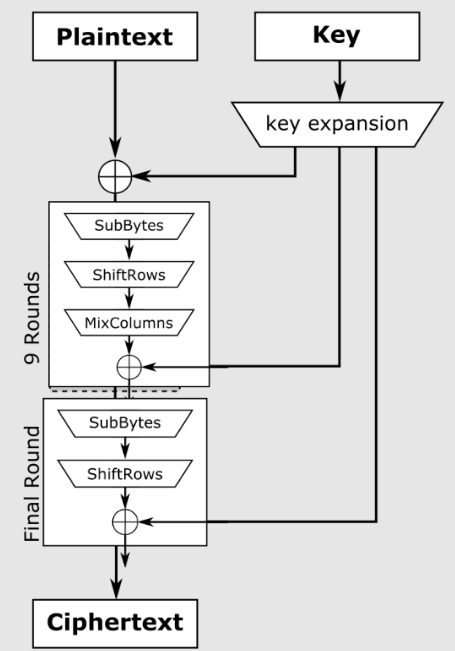
\includegraphics[width=0.5\textwidth]{figures/fig06-aes}
    \centering
    \caption{AES}
\end{figure}

Sei $b$ die Blocklänge des Ciphers. AES operiert auf einem State:
\begin{itemize}
    \item 2-dimensionales Bytearray mit 4 Zeilen und $b/32$ Spalten
    \item Sowohl Klartext als auch Schlüssel werden zu Beginn auf je ein solches Array gemappt
    \item Beispiel: bei 128 Bit Blocklänge ergibt sich ein $4 \times 4$ Array
\end{itemize}

\paragraph{Sub-Bytes} ist die einzige nicht-lineare Operation in AES. (? Todo: \verb|folien AK_02_block_v02.pdf|, Seite 65)

\begin{itemize}
    \item Konfusion
    \item S-Box 
    \item Die einzelnen Bytes werden als Elemente von $GF(2^8)$ betrachtet
    \item Irreduzibles Polynom ist $x^8 + x^4 + x^3 + x + 1$
    \item Jedes Byte $a_{i,j}$ wird transformiert zu $b_{i,j} = Sbox(a_{i, j}) = f(g(a_{i,j}))$ mittels 
    \begin{itemize}
        \item $g: a \mapsto a' = a^{-1}$
        \item $f: a' \mapsto b = A\cdot a' + v$
    \end{itemize}
    \item Affine Transformation mit $v$ um Attacken zu Vermeiden. 
\end{itemize}

\begin{equation*}
    A = \begin{pmatrix}
        1 & 1 & 1 & 1 & 1 & 0 & 0 & 0\\
        0 & 1 & 1 & 1 & 1 & 1 & 0 & 0\\
        0 & 0 & 1 & 1 & 1 & 1 & 1 & 0\\
        0 & 0 & 0 & 1 & 1 & 1 & 1 & 1\\
        1 & 0 & 0 & 0 & 1 & 1 & 1 & 1\\
        1 & 1 & 0 & 0 & 0 & 1 & 1 & 1\\
        1 & 1 & 1 & 0 & 0 & 0 & 1 & 1\\
        1 & 1 & 1 & 1 & 0 & 0 & 0 & 1\\
\end{pmatrix} \text{ und } v = (0,1,1,0,0,0,1,1)^\top
\end{equation*}

\paragraph{ShiftRows}

Diffusion:
\begin{itemize}
    \item Jede Zeile des States wird zyklisch nach links geshiftet
    \item Offsets: 0,1,2,3 für 128 Bit Blocklänge
    \item Mit diesen Offsets maximale Diffusion und größte Resistenz gegen bekannte Attacken
\end{itemize}

(todo: add graphic)

\paragraph{MixColumns}

Diffusion
\begin{itemize}
    \item Arbeitet auf den Spalten des States (wegen 32-Bit Architektur sind 4 Zeilen, d.h. 32 Bit pro Spalte optimal)
    \item Bytes einer Spalte werden Koeffizienten eines Polynoms vom Grad 3 in $GF(2^8)$ betrachtet
    \begin{itemize}
        \item Spalte wird multipliziert mit $03x^3 + 01x^2 + 01x + 02$
        \item Multiplikation mit 01 ist die Identität 
        \item Multiplikation mit 02 ist ein Shift und ein XOR 
        \item Multiplikation mit 03 ist eine Multiplikation mit 02 und ein XOR 
        \item Reduziert mit $x^4 + 1$ 
    \end{itemize}
\end{itemize}

De facto handelt es sich also um ein Polynom in $x$, dessen Koeffizienten Polynome sind. Herleitung daher allgemein einfacher.
Notation: statt $a_{i,j}$ steht im Folgenden $a_i$, zur Wahrung der Übersichtlichkeit. \\

Beispiel: Stelle 

\begin{align*}
    (02a_3+a_2+a_1+03a_0)&x^3 + \\
    (03a_3+02a_2+a_1+a_0)&x^2 + \\
    (a_3+03a_2+02a_1+a_0)&x^1 + \\ 
    (a_3+a_2+03a_1+02a_0)& 
\end{align*}
    
    als Matrix dar:

\begin{equation*}
    \begin{pmatrix}
        b_0 \\ b_1 \\ b_2 \\ b_3 \\
\end{pmatrix}  = \begin{pmatrix}
        02 & 03 & 01 & 01 \\
        01 & 02 & 03 & 01 \\
        01 & 01 & 02 & 03 \\
        03 & 01 & 01 & 02 \\
\end{pmatrix} \cdot \begin{pmatrix}
        a_0 \\ a_1 \\ a_2 \\ a_3 \\
\end{pmatrix} 
\end{equation*}

\paragraph{AddRoundKey}

Aktueller Rundenschlüssel wird byteweise mit aktuellem State verxort

\paragraph{Key Schedule}

Aus initialem 128-bit (bzw. 192 bzw. 256-bit) Key muss für jede
Runde ein Schlüssel in Blocklänge (128 Bit) generiert werden. Seo $b$ die Blocklänge und $r$ die Rundenanzahl.
Die zwei Schritte dafür sind:

\begin{enumerate}
    \item Key Expansion: wie wird aus initialem Schlüssel ein Schlüssel der Länge $(r + 1) \cdot b$ Bit
    \item Round Key Selection: wie wird Schlüsselteil für aktuelle Runde ausgewählt
\end{enumerate}


\begin{itemize}
    \item Schlüssel wird in 2-dimensionales Array geschrieben
    \item Die letzte Spalte des Arrays wird einmal zirkulär nach oben geshiftet
    \item Danach mittels S-Box aus SubBytes behandelt
    \item Dann mit Rundenkonstante verxort
    \begin{itemize}
        \item Runde 1: 0x01 (1, 01)
        \item Runde 2: 0x02 (x, 10)
        \item Runde 3: 0x04 (x2, 100)
        \item Runde 4: 0x08 (x3, 1000)
        \item Runde 5: 0x10 (x4, 1 0000)
        \item Runde 6: 0x20 (x5, 10 0000)
        \item Runde 7: 0x40 (x6, 100 0000)
        \item Runde 8: 0x80 (x7, 1000 0000)
        \item Runde 9: 0x1b (x8 mod (x8 + x4 + x3 + x + 1), 1 1011)
        \item Runde 10: 0x36 (x9 mod (x8 + x4 + x3 + x + 1), 11 0110)
    \end{itemize}
    \item Schließlich mit erster Spalte des letzten Rundenschlüssels verxort, ergibt erste Spalte des aktuellen Rundenschlüssels
    \item Übrige Spalten entstehen durch verxoren der vorherigen Spalte mit der entsprechenden Spalte des letzten Rundenschlüssels
(Spalte 2 des neuen Schlüssels ist also Spalte 1 des neuen verxort mit Spalte 2 des alten) 
\end{itemize}

\subsection{Entschlüsselung}

Für die Entschlüsselung brauchen wir für jede Funktion der Verschlüsselung ein Inverses:

\begin{center}
    \begin{tabular}{ ll } 
        \hline
        Verschlüsselung & Entschlüsselung \\ 
        \hline
        SubBytes & InvSubBytes \\
        ShiftRows & InvShiftRows \\
        MixColumns & InvMixColumns \\
        AddRoundKey & AddRoundKey (selbstinvers) \\
        \hline
    \end{tabular}
\end{center}

Weiters, muss die Reihenfolge der Operationen umgekehrt werden.
Möglichkeit einer mathematisch äquivalenten Beschreibung, um die Reihenfolge beizubehalten:

\begin{itemize}
    \item InvSubBytes und InvShiftRows können vertauscht werden, es ist völlig egal, ob Werte zuerst ersetzt und dann verschoben werden, oder umgekehrt
    \item InvMixColumns und AddRoundKey können vertauscht werden, weil InvMixColumns linear ist, d.h. $F(a\oplus b) = F(a) \oplus F(b)$
\end{itemize}

\noindent Damit ist wenn EquivRoundKey := InvMixColumns(RoundKey):

$$\text{InvMixColumns}(\text{State} \oplus \text{Roundkey}) = \text{InvMixColumns}(\text{State}) \oplus \text{EquivRoundKey}.$$ 

\paragraph{Beispiel} für 3 Runden:

\begin{center}
    \begin{tabular}{ lll } 
        \hline
        Verschlüsselung & $>$ Entschlüsselung & $>$ Entschlüsselung optimiert\\ 
        \hline
        AddRoundKey & AddRoundKey   & AddRoundKey \\
        SubBytes    & InvShiftRows  & InvSubBytes \\
        ShiftRows   & InvSubBytes   & InvShiftRows \\ 
        MixColumns  & AddRoundKey   & InvMixColumns \\
        AddRoundKey & InvMixColumns & EquivRoundKey \\
        SubBytes    & InvShiftRows  & InvSubBytes \\
        ShiftRows   & InvSubBytes   & InvShiftRows \\
        MixColumns  & AddRoundKey   & InvMixColumns \\
        AddRoundKey & InvMixColumns & EquivRoundKey \\
        SubBytes    & InvShiftRows  & InvSubBytes \\
        ShiftRows   & InvSubBytes   & InvShiftRows \\
        AddRoundKey & AddRoundKey   & AddRoundKey \\
        \hline
    \end{tabular}
\end{center}

\subsection{Zusammenfassung}

\paragraph{Effizienz}

\begin{itemize}
    \item Sämtliche Berechnungen können vorab als Lookup-Tables gespeichert werden
    \item SubBytes, ShiftRows und MixColumns können in einer Operation zusammengefasst werden
    \item Sowohl in Hardware als auch in Software schnell implementierbar
    \item Von 8-bit bis 128-bit Architekturen
    \item Intel mit eigenen Instruction Set Extensions für AES (z.B. \verb|AESENC|, \verb|AESENCLAST|, \verb|AESDEC|, \ldots)
\end{itemize}

\paragraph{Designentscheidungen}

\begin{itemize}
    \item Anzahl der Runden
    \begin{itemize}
        \item Volle Diffusion nach 2 Runden (mit Feistelnetzwerk nicht erreichbar)
        \item Änderung in einem State Bit beeinflusst ungefähr die Hälfte aller State Bits nach 2 Runden
        \item Keine Attacken für Versionen ab 6 Runden gefunden
        \item 4 Runden Security Margin hinzugefügt, damit also quasi je einmal volle Diffusion am Anfang und am Ende hinzugefügt
        \item Für je 32 Bit Schlüssellänge wird eine Runde hinzugefügt
        \item Für je 32 Bit Blocklänge wird eine Runde hinzugefügt (betrifft nur Rijndael)
    \end{itemize}
    \item SubBytes
    \begin{itemize}
        \item ist nicht-linear, erreicht durch Inversion in endlichem Körper
        \item Algebraisch Komplex, erreicht durch affine Transformation
    \end{itemize}
    \item ShiftRows
    \begin{itemize}
        \item Maximale Diffusion (4 unterschiedliche Offsets)
        \item Einfachste Variante bei mehreren gleichwertigen gewählt
    \end{itemize}
    \item MixColumns
    \begin{itemize}
        \item 4-Byte Spalten, um 32-Bit Architektur auszunützen
        \item Linear in $GF(2)$
        \item Diffusion, nicht zwangsläufig optimale
        \item Auch auf 8-Bit Architekturen gute Performance
    \end{itemize}
    \item KeyAddition und Key Schedule
    \begin{itemize}
        \item Durch Addition des Keys am Anfang und am Ende (siehe Whitening)
        \item Möglichst wenig Arbeitsspeicher für KeyExpansion durch rekursive Definition
        \item Symmetrien eliminiert durch Addition der Rundenkonstanten
        \item Diffusion
    \end{itemize}
\end{itemize}

\paragraph{Kritik und Angriffe}

Es gibt zwei große Kritikpunkte bzgl. AES: 

\begin{itemize}
    \item Einfachheit
    \begin{itemize}
        \item Großteil ist algebraisch zu beschreiben
        \item Ungewöhnlich für Blockcipher
    \end{itemize}
    \item Key Schedule 
    \begin{itemize}
        \item Attacken für 256 Bit Keys bekannt
    \end{itemize}
\end{itemize}

Die momentan besten Angriffe sind:

\begin{itemize}
    \item Auf AES-256, 14 Runden, in $O(2^{99.5})$
    \item Auf AES-192, 12 Runden, in $O(2^{176})$
    \item Auf AES-128, 10 Runden, in $O(2^{126.1})$
\end{itemize}


\section{Streamchipher}\index{Streamchipher}

Im Gegensatz zu Blockciphern werden hier Daten verschlüsselt, sobald sie zur
Verfügung stehen. Das wird überall dort gebraucht, wo Latenzen ein Problem bereiten.\\ 

\noindent Streamciphers sind üblicherweise sehr effizient in Hardware implementierbar. \\

\noindent Datenstrom wird mit einem Schlüsselstrom\index{Schlüsselstrom}\index{Keystream} verknüpft (üblicherweise per xor)m dafür muss der Schlüsselstrom gleich lang 
sein wie die Daten.
Im Idealfall ist der Schlüsselstrom eine komplette Zufallsfolge (siehe One-Time Pad). \\

\noindent Bei Streamciphern sind Konfusion und Diffusion nicht möglich. Das heißt die Sicherheit liegt allein in der Qualität des Schlüsselstroms. \\

\noindent Streamcipher werden sehr oft gerade in der Telekommunikationsbranche verwendet,
allerdings gibt es sehr wenige Spezifikationen die öffentlich oder standardisiert sind. Eine Initiative, die versucht eine Standardisierung zu erreichen war z.B. das
eSTREAM Projekt der EU. \\

\noindent Durch geeigneten Betriebsmodus kann beliebiger Blockcipher zu Streamcipher umgebaut werden. Damit sind grundsätzlich alle positiven, untersuchten Eigenschaften des
Blockciphers auf den erzeugten Schlüsselstrom übertragbar.

\subsection{Streamchipher Modi}\index{Streamcipher Modi}

\paragraph{CFB (Cipher Feedback Mode)}\index{Streamcipher Modi!CFB}\index{CFB}

\begin{align*}
    c_i = p_i \oplus E_K(c_{i-1}) \\
    p_i = c_i \oplus E_K(c_{i-1})
\end{align*}

Vorteile: 
\begin{itemize}
    \item selbstsynchronisierend (self-synchronizing): wenn $n$ Bit gleichzeitig verschlüsselt werden, hängt der Keystream\index{Schlüsselstrom!CFB}\index{Keystream!CFB} 
    nur von den letzten $n$ Bit ab
\end{itemize}

Nachteile: 
\begin{itemize}
    \item 1 Bit Fehler im $i$-ten Ciphertext verursacht zuerst 1 Bit Fehler im $i$-ten Klartext, danach
fehlerhaften folgenden $(i+1)$-ten Block
    \item Angreifer kann beliebige Bits manipulieren. Der folgende Block lässt sich danach nicht
mehr entschlüsseln, je nach Applikation kann das dem Angreifer aber genügen. 
    \item Der letzte Block lässt sich völlig unbemerkt manipulieren
    \item Wie im CBC Mode wird ein IV benötigt, dieser muss aber einzigartig sein, ansonsten
entstehen gleiche Keystreams\index{Schlüsselstrom!CFB}\index{Keystream!CFB}
\end{itemize}


\paragraph{OFB (Output Feedback Mode)}\index{Streamcipher Modi!OFB}\index{OFB}

Sei $s_i = E_K(s_{i-1})$, dann

\begin{align*}
    c_i = p_i \oplus s_i  \\
    p_i = c_i \oplus s_i
\end{align*}

Vorteile: 
\begin{itemize}
    \item $s_i$ ist unabhängig von Klar- und Ciphertext, d.h. Schlüsselstrom\index{Schlüsselstrom!OFB}\index{Keystream!OFB} beliebiger Länge kann offline vorberechnet 
    werden (synchronous)
    \item 1 Bit Fehler im Ciphertext bewirkt nur 1 Bit Fehler im Klartext, keine Fehlerfortpflanzung
\end{itemize}


Nachteile: 
\begin{itemize}
    \item Synchronisation wichtig; sobald beide Schlüsselströme\index{Schlüsselstrom!OFB}\index{Keystream!OFB} nicht mehr synchron laufen, keine Entschlüsselung mehr 
    möglich
    \item Insertion Attack möglich
\end{itemize}

\subparagraph{Insertion Attack}
\begin{enumerate}
    \item Angenommen, Angreifer kennt Ciphertextstream $c = (c_1, c_2, c_3, \ldots)$ 
    \item Es gilt, $c$ entstand durch xor von Klartextstream $p$ und Schlüsselstream\index{Schlüsselstrom!Insertion Attack}\index{Keystream!Insertion Attack} 
    $k$ ($c_1 = p_1 \oplus k_1, \ldots$)
    \item Angreifer fügt Bit $p_1'$ in $p$ ein (z.B. nach $p_1$) und schneidet neuen Cipherstream mit
    \item Wenn derselbe Keystream\index{Schlüsselstrom!Insertion Attack}\index{Keystream!Insertion Attack} verwendet wurde, dann gilt:
    \begin{itemize}
        \item $c_1 = p_1 \oplus k_1$
        \item $c_2' = p_1' \oplus k_2$ 
        \item $c_3' = p_2 \oplus k_3$
        \item \ldots
    \end{itemize}
    \item Da Angreifer $p_1'$ kennt, kann er alle darauffolgenden Bits und in Folge den kompletten Keystream\index{Schlüsselstrom!Insertion Attack}
    \index{Keystream!Insertion Attack} entschlüsseln:
    \begin{itemize}
        \item $k_2 = c_2' \oplus p_1'$
        \item $p_2 = c_2 \oplus k_2$
        \item $k_3 = c_3' \oplus p_2$
        \item \ldots
    \end{itemize}

\end{enumerate}

\paragraph{CTR (Counter Mode)}\index{Streamcipher Modi!CTR}\index{CTR}

Sei $s_i = E_K(\text{Nonce}||i)$, dann 

\begin{align*}
    c_i = p_i \oplus s_i \\
    p_i = c_i \oplus s_i
\end{align*}

Vorteile: 
\begin{itemize}
    \item $s_i$ kann parallel berechnet werden, kein Feedback nötig
    \item Nonce $|| i$ muss Blocklänge haben (also z.B. 128-Bit bei AES)
    \item Wahlfreier Zugriff
    \item Sehr einfach
\end{itemize}

Nachteile: 
\begin{itemize}
    \item Bit Flipping möglich
    \item Nonce und Zähler dürfen nicht mehrmals verwendet werden
\end{itemize}

\paragraph{GCM (Galois Counter Mode)}\index{Streamcipher Modi!GCM}\index{GCM}

TODO

\begin{align*}
    y_0 &= IV||1 \\ 
    H &= E_K(0) \\
    GHASH(H,A,C) &= \bigoplus_i \left((A_i \bullet H^i ) \oplus \left(\bigoplus_j (C_{j+i} \bullet H^{j+i} )\right)\right)\ldots\\
    T &= GHASH(H,A,C) \oplus E_K(y_0) \\
\end{align*}

und $si = E_K(y_{i-1}+1)$, dann ist die Definition der Ver- und Entschlüsselung

\begin{align*}
    c_i = p_i \oplus s_i \\
    p_i = c_i \oplus s_i
\end{align*}

Vorteile: 
\begin{itemize}
    \item $s_i$ kann parallel berechnet werden, kein Feedback nötig
    \item $T$ dient als Authentication Tag, authentifiziert den Ciphertext
    \item $A$ sind Daten, die nur authentifiziert, nicht verschlüsselt werden
    \item Sehr schnell in Hard- und Software
\end{itemize}

Nachteile: 
\begin{itemize}
    \item IV darf nur einmal verwendet werden
\end{itemize}

\subsection{Klassifikation}

\paragraph{One-Time Pad}\index{One-Time Pad}

Ein One-Time Pad ist unconditionally secure. Hierbei ist der Schlüssel genauso lang wie die Nachricht und absolut zufällig.

\paragraph{Synchron}

Ein Keystream\index{Schlüsselstrom!One-Time Pad}\index{Keystream!One-Time Pad} wird unabhängig von der Nachricht erzeugt und hängt nur vom initialen Schlüssel und dem 
aktuellen internen Zustand des Ciphers ab (z.b. OFB).
Der Sender und Empfänger müssen daher stets im selben internen Zustand sein, d.h. eine externe Synchronisation ist notwendig.
Bei dieser Art gibt es keine Fehlerfortpflanzung.

\paragraph{Asynchron (selbstsynchronisierend)}

Der Keystream\index{Schlüsselstrom!One-Time Pad}\index{Keystream!One-Time Pad} ist eine Funktion des Schlüssels und der letzten $n$ Ciphertext Zeichen (z.B. CFB).
Bei fehlenden/eingefügten Zeichen pflanzt sich der Fehler nur über $n$ Zeichen fort,
danach synchronisiert sich der Empfänger von selbst wieder.

\subsection{Exkurs: AEAD (Authenticated Encryption with Associated Data)}\index{AEAD}\index{Authenticated Encryption with Associated Data} 

AEAD bezeichnet einen Cipher Modus, der gleichzeitig (simultan!) Confidentiality und Authenticity bereitstellt. Es fügt einer verschlüsselten Nachricht einen 
Authentifizierungs-Tag an, der den Besitz des privaten Schlüssel garantiert. Beispiele für Algorithmen, die AEAD ermöglichen sind AES-GCM oder ChaCha20-Poly1305. \\

\noindent In vielen modernen Protokollen wird AEAD verwendet, z.B. TLS1.3, HTTP3 und VPNs.

\subsection{ChaCha20}

Der ChaCha20 wurde 2008 von Daniel J. Bernstein entwickelt und wird in RFC 8439 beschrieben. Er ist eine verbesserte Version des Salsa20 Ciphers.
Er ist schnell, sicher und einfach zu implementieren und hat breite Verwendung gefunden, z.B.: 

\begin{itemize}
    \item TLS
    \item SSH 
    \item VPNs 
    \item Android 
    \item \ldots
\end{itemize}

\noindent Für diesen Cipher sind keine praktischen Angriffe bekannt, er ist sogar resistent gegen Timing-Angriffe.\\

\noindent Die Runden, die in der Berechnung durchlaufen werden, sorgen für eine gute Diffusion. \\

\noindent Der ChaCha20 wird häufig in Kombination mit dem Authentifizierungsalgorithmus Poly1305  verwendet, das ChaCha20-Poly1305 AEAD\index{AEAD}. \\

\noindent Weitere Infos auf \url{https://cr.yp.to/chacha.html}.

\paragraph{Beschreibung} \mbox{} \\

Inputs:
\begin{itemize}
    \item Key (256 Bit, d.h. 32 Byte)
    \item Nonce bzw. IV (96 Bit)
    \item Counter (32 Bit)
\end{itemize}

\noindent Zwei Nachrichten mit demselben Key dürfen nicht den gleichen Ciphertext erzeugen. Der Counterwird pro 64-Byte-Block erhöht. \\

\noindent Output: Keystream\index{Schlüsselstrom!ChaCha20}\index{Keystream!ChaCha20}, der aus Key, Nonce und Counter erzeugt wird und mit dem Plaintext verxort den Ciphertext stream ergibt.\\

Es gibt einen internen 512-Bit-State, der aus 16 ($4\times 4$) 32-Bit-Wörtern besteht:
\begin{itemize}
    \item 0-3: Konstante (``expand 32 byte k'')
    \item 4-11: 256 Bit Schlüssel 
    \item 12: Counter
    \item 13-15: Nonce
\end{itemize}

Es werden 20 Runden (10 Double Rounds) einer Add-XOR-Rotation durchgeführt. Eine Quarter Round (mit 4 von 16 Wörtern) führt aus:

\begin{minipage}[c]{0.48\textwidth}
        \verb|a += b; d ^= a; d <<< 16;| \\
        \verb|c += d; b ^= c; b <<< 12;| \\
        \verb|a += b; d ^= a; d <<< 8;| \\
        \verb|c += d; b ^= c; b <<< 7;|
\end{minipage} \begin{minipage}[c]{0.48\textwidth}
    \centering
    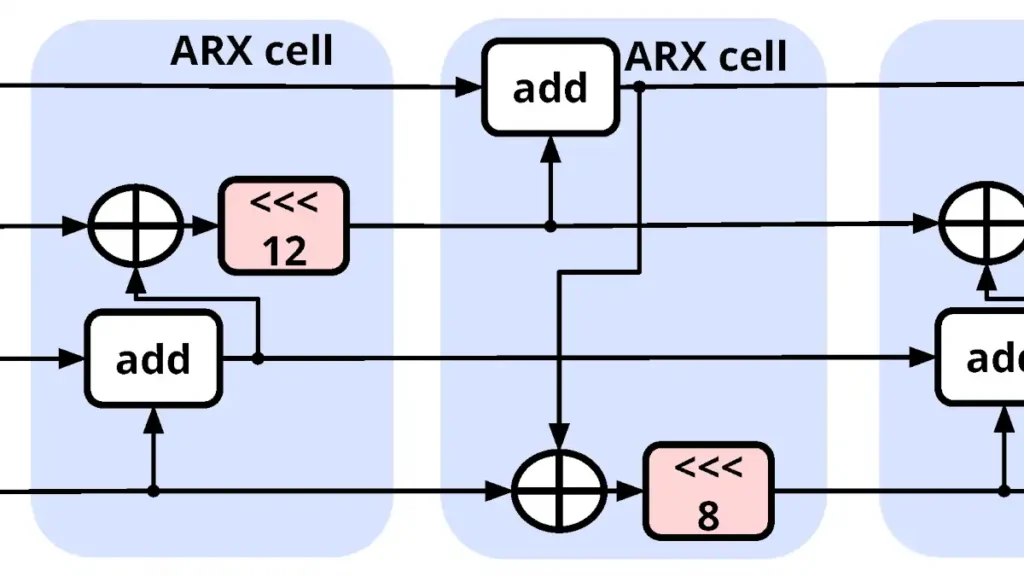
\includegraphics[width=0.9\textwidth]{figures/fig07-chacha20-1024x576.png}
\end{minipage}


\chapter{Padding}\index{Padding}

Bei allen Algorithmen, die Nachrichten in festen Blöcken verarbeiten, muss die Nachrichtenlänge
ein Vielfaches der Blocklänge sein. Das gilt z.B. bei Blockciphern, aber auch bei Hashfunktionen etc. \\

\noindent Manchmal hilft Padding auch bei der Verschleierung des tatsächlichen Inhalts bei deterministischen Verfahren wie z.B. RSA oder klassische Cipher. \\

\noindent Deswegen versuchen wir, unsere Nachrichten in einer passenden Form aufzufüllen. Entweder weiß der Empfänger über das Padding Bescheid, oder er kann es - je nach konkreter 
Anwendung ignorieren. Es ist aber zu beachten, dass das Padding sich klar von der Nachricht untescheidet. Ein Negativbeispiel ist das Padding mit zufälligen Wörtern und 
Sätzen, wie bei der Geschichte aus dem zweiten Weltkrieg: \url{https://en.wikipedia.org/wiki/The_world_wonders}. \\

\noindent Es gilt zwar, dass ein Padding eine Nachricht immer verlängert, wir versuchen diese aber auf weniger als eine Blockgröße zu beschränken.

\section{Block cipher mode of operation}

Bei einem einfachen Padding, könnte der letzte Block mit einem regulären Bitmuster aufgefüllt werden:

\begin{itemize}
    \item nur 0er bzw. nur 1er
    \item abwechselnd 0 und 1
    \item so, dass der Empfänger das Padding entfernen kann
    \begin{itemize}
        \item z.B. lauter 0er und am Ende ein Byte, das angibt, wie viele Bytes entfernt werden sollen (z.B. \ldots, \verb|0x12, 0x15, 0x0, 0x0, 0x2|)
        \item dann muss aber jede Nachricht gepadded werden
        \item im schlimmsten Fall, muss ein gesamter Block angefügt werden
    \end{itemize}
\end{itemize}

Bei CBC gibt es folgendes Schema:

\begin{enumerate}
    \item Der letzte vollständige Block wird nochmals verschlüsselt
    \item Die linkesten $l$ Bit des neuen Ciphertext Blocks werden mit dem $l$-bit langen Klartextrest verxort
    \item Problem: Angreifer kann durch Manipulation des Ciphertextes gezielt Bits im letzten Klartextblock verändern
\end{enumerate}

\paragraph{Cipher Text stealing}\index{Cipher Text Stealing}

\begin{center}
    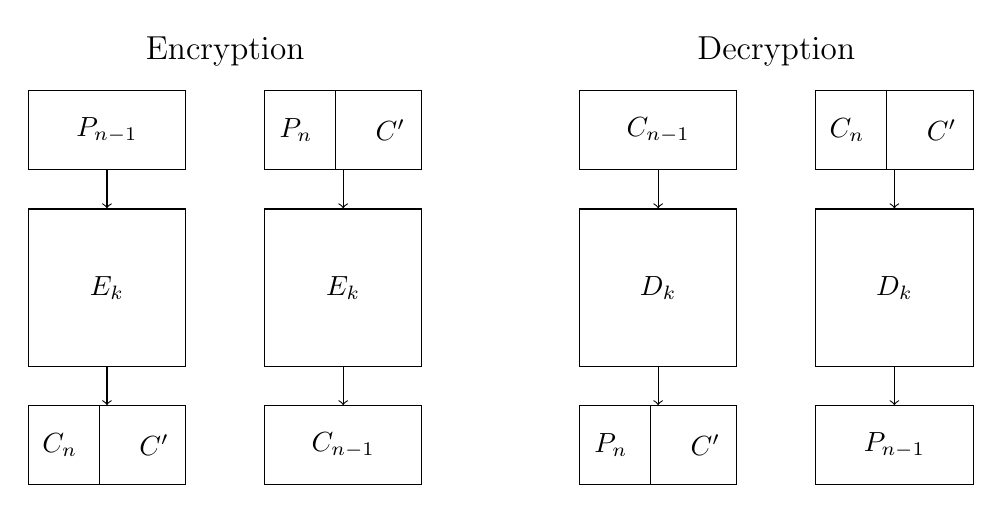
\begin{tikzpicture}[node distance=1cm and 1.5cm, every node/.style={align=center}]
      % Encryption Title
      \node (title1) [font=\large] at (-5,5) {Encryption};

      % Encryption - Left side
      \node (pn1) [draw, minimum width=2cm, minimum height=1cm] at (-6.5,4) {$P_{n-1}$};
      \node (ek1) [draw, minimum width=2cm, minimum height=2cm] at (-6.5, 2) {$E_k$};
      \node (cdash1) at (-5.9, 0) {$C'$};
      \node (cn1) at (-7.1, 0) {$C_n$};
      \node (auxc1) [draw, minimum width=2cm, minimum height=1cm] at (-6.5, 0) {};
      \draw (-6.6, 0.5) -- (-6.6, -0.5);
      \draw[->] (pn1) -- (ek1);
      \draw[->] (ek1) -- (auxc1);

      % Encryption - Right side
      \node (auxp1) [draw, minimum width=2cm, minimum height=1cm] at (-3.5, 4) {};
      \node (pn2) at (-4.1, 4) {$P_n$};
      \node (cdash2) at (-2.9, 4) {$C'$};
      \node (ek2) [draw, minimum width=2cm, minimum height=2cm] at (-3.5, 2) {$E_k$};
      \node (cn2) [draw, minimum width=2cm, minimum height=1cm] at (-3.5,0) {$C_{n-1}$};
      \draw (-3.6, 3.5) -- (-3.6, 4.5);
      \draw[->] (auxp1) -- (ek2);
      \draw[->] (ek2) -- (cn2);

      % Decryption Title
      \node (title2) [font=\large] at (2,5) {Decryption};

      % Decryption - Left side
      \node (cpn1) [draw, minimum width=2cm, minimum height=1cm] at (0.5,4) {$C_{n-1}$};
      \node (dek1) [draw, minimum width=2cm, minimum height=2cm] at (0.5, 2) {$D_k$};
      \node (dcdash1) at (1.1, 0) {$C'$};
      \node (dpn1) at (-0.1, 0) {$P_n$};
      \node (dauxc1) [draw, minimum width=2cm, minimum height=1cm] at (0.5, 0) {};
      \draw (0.4, 0.5) -- (0.4, -0.5);
      \draw[->] (cpn1) -- (dek1);
      \draw[->] (dek1) -- (dauxc1);

      % Decryption - Right side
      \node (dauxp1) [draw, minimum width=2cm, minimum height=1cm] at (3.5, 4) {};
      \node (dcn2) at (2.9, 4) {$C_n$};
      \node (dcdash2) at (4.1, 4) {$C'$};
      \node (dek2) [draw, minimum width=2cm, minimum height=2cm] at (3.5, 2) {$D_k$};
      \node (dpn2) [draw, minimum width=2cm, minimum height=1cm] at (3.5,0) {$P_{n-1}$};
      \draw (3.4, 3.5) -- (3.4, 4.5);
      \draw[->] (dauxp1) -- (dek2);
      \draw[->] (dek2) -- (dpn2);

    \end{tikzpicture}
\end{center}

Bei Cipher Text Stealing wird der vorletzte komplette Block $P_{n-1}$ verschlüsselt und in Teile $C_n$ und $C'$ aufgeteilt. 
Dann wird der letzte Block $P_n$ mit $C'$ gepadded und verschlüsselt. Dieser komplette Block $C_{n-1}$ kommt an die vorletzte Stelle des Ciphertexts und der noch nicht 
verwendete Teil $C_n$ wird angehängt. So kann die Nachricht mit Block Ciphern verschlüsselt werden, ohne sie zu verlängern.

\section{Hashfunktionen}\index{Padding!Hashfunktion}

\paragraph{MD5 und SHA-1} Hier muss die Nachricht um 64 Bits kleiner sein als ein Vielfaches von 512.
Das Padding ist eine 1 und entsprechend vielen 0 auf die benötigte Länge. Danach werden 64 Bit mit der Länge der ungepaddeten Nachricht angehängt, das erzeugt eine 
Nachricht mit einer durch 512 teilbaren Länge. \\

\noindent Diese Methode vermeidet, dass gleich beginnende und mit 0 endende Nachrichten denselben
Hashwert haben. Ohne das Einfügen der 1 vor dem Padding (und ohne angefügte Länge)
würden \verb|foo| und \verb|foo00| bzw. \verb|foo100| denselben Hash ergeben.

\section{Byteweise}

\paragraph{ANSI X.923} Mit 0x00 Bytes gepaddet, letztes Byte gibt Anzahl der Padding Bytes an

\paragraph{ISO 10126} Mit zufälligen Bytes gepaddet, letztes Byte gibt Anzahl der Padding Bytes
an (mittlerweile zurückgezogen)

\paragraph{ISO 7816} (ISO 9797) Ein fixes Byte markiert Beginn des
Paddings, danach mit 0x00 aufgefüllt. Im Wesentlichen bei Smartcards
verwendet.

\paragraph{PKCS5/7} (RFC3852) Letzter Block gepaddet mit $n$ Bytes, alle mit Wert $n$. Mögliche Varianten sind also
\begin{itemize}
    \item \verb|0x01|
    \item \verb|0x02 0x02|
    \item \verb|0x03 0x03 0x03|
    \item \ldots
\end{itemize}

\paragraph{Zero Padding} Mit 0x00 aufgefüllt, ist nicht reversibel

\section{RSA}\index{Padding!RSA}

Zu kurze Nachrichten problematisch zu verschlüsseln. Ursprünglich wurde einfach mit Zufallsdaten auf bestimmte Länge aufgefüllt
Im ersten Public-Key Cryptography Standards (PKCS) < v2.0:
\begin{itemize}
    \item v1.5 = RFC 2313
    \item EM = 0x00||BT||PS||0x00||M
    \item BT (Block Type) ist
    \begin{itemize}
        \item 0x00 oder 0x01 für Private Key Operationen (signieren)
        \item 0x02 für Public Key Operationen (verschlüsseln)
    \end{itemize}
    \item PS (Padding String) ist ($k$ - Länge von $M$ - 3) Bytes lang, mindestens aber 8
    \begin{itemize}
        \item k = Länge des Modulus in Byte
        \item PS ist 0x00 für BT = 0x00, 0xFF für BT = 0x01 und zufällig für BT = 0x02
    \end{itemize}
    \item Problem: nicht übermäßig zufällig, Struktur der Klartextnachricht erratbar
    \item Bleichenbacher Angriff (\url{https://web.archive.org/web/20120204040056/}, \url{http://www.bell-labs.com/user/bleichen/papers/pkcs.ps})
\end{itemize}

Mittlerweile iwrd üblicherweise Optimal Asymmetric Encryption Padding (OAEP) verwendet, eingeführt in PKCS\#1 v2.0

\section{OAEP (Optimal Asymmetric Encryption Padding)}\index{OAEP}\index{Optimal Asymmetric Encryption Padding}\index{Padding!OAEP}

\paragraph{Ablauf}

Sei $M$ eine Nachricht der Länge $m$ und $h$ die Länge des Hashes.

\begin{enumerate}
    \item Label $L$ wird gehasht, Ergebnis ist $l_{Hash}$
    \item Padding String $p$ aus 0x00 wird an $l_{Hash}$ angehängt, sodass die resultierende Länge um ($m + h + 2$) Bytes kürzer ist als der RSA Modulus in Bytes ($k$)
    \item es wird 0x01 und $M$ an den Block angehängt, daraus resultiert Data Block (DB), der um $h+1$ Bytes kürzer ist als $k$
    \begin{itemize}
        \item DB = $l_{Hash}$ || $p$ || 0x01 || $M$
    \end{itemize}
    \item Ein zufälliger String $r$ (ein sog. seed) mit Länge $h$ wird erzeugt
    \item $r$ wird mittels der Mask Generation Function (MGF) auf die Länge $(k - h - 1)$ Bytes vergrößert und mit DB verxort, das Ergebnis ist $DB_{masked}$
    \item $DB_{masked}$ wird mittels MGF auf die Länge $h$ verkleinert und mit $r$ verxort, das Ergebnis ist $r_{masked}$
    \item Encoded Message (EM) entsteht durch Konkatenation von 0x00, $r_{masked}$ und $DB_{masked}$
    \begin{itemize}
        \item EM = 0x00 || $r_{masked}$ || $DB_{masked}$
        \item Das erste 0 Byte dient dazu, zu garantieren, dass EM tatsächlich kleiner ist als der Modulus $n$: beide haben $k$ Byte, aber da in EM das höchstwertige Byte 
        0 ist, gilt sicher immer: EM $< n$.
    \end{itemize}
    \item EM wird mittels RSA verschlüsselt, d.h. $C = \text{EM}^e \mod n$
\end{enumerate}

\begin{figure}[h]
    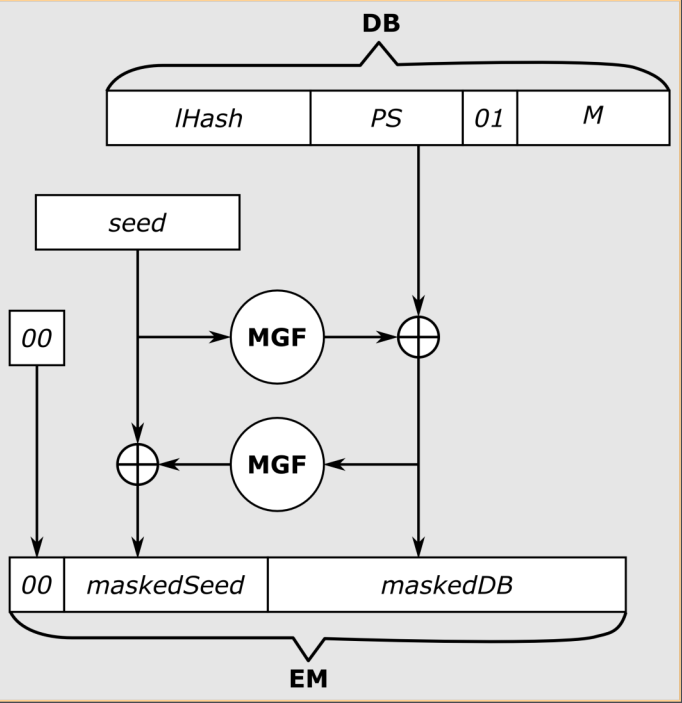
\includegraphics[width=0.4\textwidth]{figures/fig08-oaep}
    \centering
    \caption{Ablauf OAEP Verschlüsselung}
\end{figure}

\paragraph{Entschlüsselung}

\begin{enumerate}
    \item Empfänger bekommt Ciphertext $C$ und Label $L$
    \item Generiert EM aus $C$ mittels seines privaten Schlüssels, dabei muss das erste Byte von EM 0x00 sein
    \item Die nächsten $h$-Bytes sind $r_{masked}$, der Rest ($k - h - 1$) ist $DB_{masked}$
    \item $DB_{masked}$ wird mittels MGF auf Länge $h$ gebracht und mit $r_{masked}$ verxort, resultiert im Seed $r$
    \item $r$ wird mittels MGF auf Länge von $DB_{masked}$ gebracht und damit verxort, ergibt $DB$
    \item $DB$ muss beginnen mit dem Hash von $L$ (bzw. Hash des leeren Strings in PKCS\#1), gefolgt von beliebig vielen 0x00 und einer 0x01
    \item Nach 0x01 steht die Nachricht $M$
\end{enumerate}

Sowohl $DB_{masked}$ als auch $r_{masked}$ müssen vollständig bekannt sein, um $M$ zu rekonstruieren zu können. Mittels $DB_{masked}$ kann $r$ rekonstruiert werden, 
mittels $r$ dann $DB$ und in Folge $M$.
OAEP erschwert die Rekonstruktion des Klartextes für einen Angreifer. \\

\noindent Die in PKCS\#1 empfohlene Parameter für RSAES-OAEP (RSA Encryption Standard OAEP) sind 
\begin{itemize}
    \item Hash: SHA-1/256/384/512, d.h. die Hashlänge ist 20, 32, 48 oder 64 Bytes
    \item Mask Generation Function: MGF1
    \begin{itemize}
        \item $k$ Runden, in jeder Runde werden $h$ Bytes zum Output hinzugefügt, bis die gewünschte Länge erreicht ist
        \item In jeder Runde:
        \begin{itemize}
            \item 32-bit Zähler wird inkrementiert
            \item Initialwert wird mit aktuellem Zähler konkateniert und gehasht
            \item Ergebnis wird an Endergebnis angehängt
        \end{itemize}
    \end{itemize}
\end{itemize}

\chapter{Asymmetrische Kryptographie}

(todo)
% Angewandte_Kryptographie_SoSe2025_part1_v01.pdf, Seite 6ff

\section{Sicherheitsbetrachtungen von RSA}

\section{RSA in der Praxis}

\section{Mathematische Konzepte}

\subsection{Quadratischer Rest}

\subsection{Euler Kriterium und Legendre Symbol}

\subsection{Quadratwurzeln modulo $p$}

\subsection{Quadratwurzeln modulo $n = p \cdot q$}

\section{Rabin public-key encryption}

\chapter{Erzeugung von Primzahlen}

Für public-key-Kryptosysteme benötigt man häufig zufällige große Primzahlen. In der Regel erzeugt man dazu eine natürliche Zahl in der gewünschten Größe und
prüft, ob diese eine Primzahl ist, beispielsweise versucht man diese Zahl $n$ durch alle Primzahlen $\leq \sqrt{n}$ zu teilen, dieses Vorgehensweise ist jedoch sehr 
ineffizient und heißt Probedivision\index{Probedivision}. Sie wird auch in Faktorisierungsalgorithmen mit Primzahlen bis $10^6$ verwendet.

\paragraph{Verteilung der Primzahlen}

Bezeichne $\pi(n)$ die Anzahl der Primzahlen im Intervall $[2, n]$. Es gilt 

$$\pi(n) \sim \frac{n}{\ln(n)} $$


\begin{center}
    \begin{tabular}{ ll } 
        \hline
        $n$ & $\pi(n)$  \\ 
        \hline
                 10 &         4 \\
                100 &        25 \\
               1000 &       168 \\
              10000 &      1229 \\
             100000 &      9592 \\
            1000000 &     78498 \\
           10000000 &    664579 \\
          100000000 &   5761455 \\
         1000000000 &  50847534 \\
        10000000000 & 455052512 \\
        \hline
    \end{tabular}
\end{center}

\paragraph{Abschätzung des Aufwands}

Aus $\pi(n) \sim n / \ln(n)$ folgt: man benötigt wenigstens $\sqrt{n} / \ln(\sqrt{n})$ Probedivisionen, um zu
beweisen, daß eine natürliche Zahl $n$ eine Primzahl ist.
Beispielsweise werden bei RSA Primzahlen verwendet, die aktuell in der Regel größer als
$10^{150}$ sind.\\

Um nun die Primalität für diese Zahl zu beweisen, müßte man insgesamt mehr als
$10^{150/2} / \ln(10^{150/2}) > 5.7 \cdot 10^{72}$ Probedivisionen durchführen -- das ist nicht durchführbar!
Somit sucht man nach effizienteren Verfahren: Primzahltests\index{Primzahltest} stellen mit einer
hohen Wahrscheinlichkeit fest, ob eine Zahl auch eine Primzahl ist (probabilistic primality
tests).
% Angewandte_Kryptographie_SoSe2025_part1_v01.pdf, Seite 34ff

\section{Der Fermat Test}
Der Fermat-Test
- der Test beruht auf dem kleinen Satz von Fermat: Ist n eine Primzahl, so gilt 

$$a^{n-1} \equiv 1  \mod n$$ 

für alle $a \in \mathbb{Z}$ mit gcd($a,n$) = 1.

Somit kann man mit diesem Satz überprüfen, ob eine Zahl zusammengesetzt ist:

\begin{enumerate}
    \item man wählt dazu eine natürliche Zahl $a \in \{1,2, \ldots, n-1\}$
    \item als nächste berechnet man $r = a^{n-1} \mod n$
    \item ist nun $r \neq 1$, so ist $n$ keine Primzahl und zusammengesetzt. Ergibt sich $r = 1$, so kann $n$ eine Primzahl oder zusammengesetzt sein
    \item die Schritte 1 bis 3 müssen für alle Werte von $a$ nun durchlaufen werden, wenn $r = 1$
\end{enumerate}

Es braucht die Festlegung einer ``Sicherheits-Grenze'': Wie oft muss der Algorithmus bei $r = 1$ durchlaufen werden, damit man sicher sein kann, eine Primzahl gefunden 
zu haben?\\
    
\noindent Der Fermat-Test kann zeigen, dass $n$ zusammengesetzt ist, er kann aber nicht beweisen, dass $n$ eine Primzahl ist. \\

\noindent Das Verfahren ist zur Faktorisierung ungeeignet.

\paragraph{Beispiel}
Gegeben: $n = 341 = 11 \cdot 31$,  d.h. $n$ ist keine Primzahl. Wir berechnen für $a = 2$

$$2^{340} \equiv 1 \mod 341,$$

obwohl $n$ zusammengesetzt ist. Für ein anderen $a$, z.B. $a = 3$ haben wir 

$$3^{340} \equiv 56 \mod 341.$$

Im Ergebnis bedeutet das, dass 341 also eine zusammengesetzte Zahl ist und somit nicht prim sein kann.

\section{Carmichael-Zahlen}

Wenn der Fermat-Test für viele Basen $a$ keine Bestätigung für ein zusammengesetztes $n$
gefunden hat, ist es wahrscheinlich, dass $n$ eine Primzahl ist.
Es existieren aber natürliche Zahlen, deren Eigenschaft ist, dass sie zusammengesetzt sind,
das jedoch nicht mit dem Fermat-Test gezeigt werden kann. \\

Sei $n$ eine ungerade zusammengesetzte Zahl und es gilt für eine ganze Zahl $a$ folgende
Kongruenz

$$a^{n-1} \equiv 1 \mod n,$$

so nennt man $n$ eine Pseudoprimzahl zur Basis $a$. Sei $n$ nun eine Pseudoprimzahl zur Basis $a$ für alle ganzen Zahlen $a$ mit gcd($a,n$) = 1. Dann
heißt $n$ Carmichael-Zahl\index{Carmichael-Zahl}. 

\paragraph{Beispiel} für eine Carmichael-Zahl: $561 = 3 \cdot 11 \cdot 17$.

\paragraph{Eigenschaften} Eine ungerade zusammengesetzte Zahl $n \geq 3$ ist eine Carmichael-Zahl, wenn genau
diese zwei Bedingungen gelten:
\begin{enumerate}
    \item $n$ ist quadratfrei, d.h. $n$ hat keinen mehrfachen Primteiler
    \item $p - 1$ teilt $n - 1$ für alle Primteiler $p$ von $n$
\end{enumerate}

Somit folgt, dass jede Carmichael-Zahl ein Produkt von mindestens drei unterschiedlichen
Primzahlen ist. Daher wissen wir auch, dass unendlich viele Carmichael-Zahlen existieren.

\section{Der Miller-Rabin Test}

Im Gegensatz zum Fermat-Test findet der Miller-Rabin-Test nach ``ausreichend'' vielen
Durchläufen für jede natürliche Zahl heraus, ob diese zusammengesetzt ist. \\


\noindent Sei $n$ eine natürliche ungerade Zahl mit $s = \max\{r \in \mathbb{N} | 2^r \text{ teilt } n-1\}$.
Damit ist $2^s$ die größte Potenz, die $n-1$ teilt oder anders ausgedrückt: es gibt ein ungerades $d \in \mathbb{Z}$, sodass $n - 1 = 2^s \cdot d$.

\begin{theorem}
    Ist $n$ eine Primzahl und $a$ eine zu $n$ teilerfremde ganze Zahl, so gilt mit den
obigen Bezeichnungen entweder
    \begin{enumerate}
        \item $a^d \equiv 1 \mod n$
        \item$a^{2^r \cdot d} \equiv -1 \mod n$
    \end{enumerate}
\end{theorem}

Mindestens eine der Bedingungen muss erfüllt sein, dass $n$ eine Primzahl ist. Weiters gilt, $n$ ist keine Primzahl (also zusammengesetzt) g.d.w. man eine ganze zu $n$ 
teilerfremde Zahl $a$ findet, für die weder die Bedingung (1) noch (2) für ein $r \in \{0, 1, \ldots, s-1\}$ gilt.
Dann wird $a$ Zeuge gegen die Primalität von $n$ genannt.

\paragraph{Beispiel}
Sei $n = 561$ und $a = 2$. Wir behaupten $a$ ist eine Zeuge gegen die Primalität von $n$:

Wir berechnen $s = 4$ und wählen $d = 35$, dann gilt

\begin{align*}
    2^{35} &\equiv 263 \mod 561 \\
    2^{2\cdot 35} &\equiv 166 \mod 561 \\ 
    2^{4\cdot 35} &\equiv 67 \mod 561 \\
    2^{8\cdot 35} &\equiv 1 \mod 561
\end{align*}

Also ist 561 keine Primzahl nach vorhergehenden Theorem.

\paragraph{Abschätzung der Anzahl der Zeugen gegen eine Primalität einer Zahl $n$}

\begin{theorem}
Sei $n \geq 3$ eine ungerade zusammengesetzte Zahl, so gibt es in der Menge
$\{1,2, \ldots, n-1\}$ höchstens $(n-1)/4$ Zahlen, die zu $n$ teilerfremd sind und keine Zeugen gegen die
Primalität von $n$ sind.
\end{theorem}

Für einen Beweis: vgl. Buchmann J., Einführung in die Kryptographie, 3. Auflage, S. 127 ff.

\paragraph{Beispiel}: Bestimmung aller Zeugen gegen eine Primalität der Zahl $n$.
Sei $n = 15$, es ist $n-1 = 14 = 2 \cdot 7$, daraus folgt: $s = 1$ und $d = 7$. Eine zu 15 teilerfremde Zahl $a$ ist genau dann Zeuge gegen die Primzahleigenschaft
von $n$ wenn $a^7 \mod 15 \neq \pm 1$ gilt.

In einer tabellarischen Übersicht:


\begin{center}
    \begin{tabular}{ ccc ccc ccc } 
        \hline
        $a$ & 1 & 2 & 4 & 7 & 8 & 11 & 13 & 14 \\ 
        \hline
        $a^{14} \mod 15$ &  1 &  4 &  1 &  4 &  4 &  1 &  4 &  1 \\
        $a^{ 7} \mod 15$ &  1 &  8 &  4 & 13 &  2 & 11 &  7 & 14 \\ 
        \hline
    \end{tabular}
\end{center}

Die Anzahl der zu 15 teilerfremden Zahlen in $\{1, 2,\dots,14\}$, die keine Zeugen gegen die
Primalität von $n = 15$ sind, beläuft sich auf $2 \leq (15 - 1)/4 = 3.5$.

\paragraph{Anwendung} des Miller-Rabin-Tests auf eine ungerade Zahl $n$

\begin{itemize}
    \item man wählt zufällig und gleichverteilt eine Zahl aus der Menge $\{2,3,\dots, n-1\}$
    \item ist der gcd($a,n$) > 1, so ist $n$ zusammengesetzt
    \item ist der gcd($a,n$) = 1, so testet man $a^d, a^{2d}, a^{2^2d}, \ldots, a^{2^{s-1}d}$
    \item findet man nun einen Zeugen gegen die Primalität von $n$, dann wurde gezeigt, dass $n$ zusammengesetzt ist
    \item die Wahrscheinlichkeit dafür, dass $n$ zusammengesetzt ist und man keinen Zeugen findet, beläuft sich nach obigen Theorem auf höchstens $0.25$.
\end{itemize}

Ist $n$ zusammengesetzt, so findet man bei der Iteration des Miller-Rabin-Tests mit $t$ Durchläufen mit einer Wahrscheinlichkeit von höchstens $frac14t$ keinen Zeugen 
gegen die Primalität von $n$.

\paragraph{Beispiel} nach 10 Durchläufen ergibt sich eine Wahrscheinlichkeit von $frac14 10$, das entspricht ungefähr einer $0.0001$-prozentigen Wahrscheinlichkeit, 
dass man keinen Zeugen gegen die Primzahleigenschaft von $n$ findet.

\section{Verfahren zur zufälligen Wahl von Primzahlen}

Beim Verfahren für die Erzeugung einer zufälligen $k$-Bit-Primzahl: dabei wird zuerst eine zufällige und ungerade $k$-Bit-Zahl $n$ generiert.
Davon wird das erste und letzte Bit wird auf 1 gesetzt, die restlichen $k-2$ Bits werden zufällig und gleichverteilt gesetzt. 
Jetzt wird überprüft, ob $n$ eine Primzahl ist:
\begin{itemize}
    \item ist $n$ durch eine Primzahl unter einer gewissen Schranke $B$ (in der Regel wird $B = 10^6$ gesetzt) teilbar? Die Primzahlen werden in einer Tabelle vorgehalten.
    \item wird dabei kein Teiler von $n$ gefunden, so wird der Miller-Rabin-Test mit $t$ Wiederholungen ( mit $t \geq 1$ als entsprechender Sicherheitsparameter) auf $n$ 
    angewendet
    \item wird dabei kein Zeuge gegen die Primzahleigenschaft von $n$ gefunden, so gilt $n$ nun als Primzahl (mit der Sicherheit $\frac{t}{4}$).
    \item ansonsten muß der gesamte Test mit einer anderen Zahl $n'$ wiederholt werden
\end{itemize}

Die Auswahl der Schranke $B$ hängt von dem Verhältnis der Ausführungszeiten einer
Probedivision und eines Miller-Rabin-Tests auf der verwendeten Hard- bzw. Software-Plattform ab.
\chapter{Hashfunktionen}\index{Hashfunktion}

Die Anforderungen an eine kryptographische Hashfunktion sind:
\begin{itemize}
    \item Kompression, d.h. ein beliebig langer Input wird auf einen Output fixer Länge gemappt
    \item Einwegfunktion (preimage resistance), d.h. gegeben $y = h(x)$ ist es schwierig, das verwendete $x$ zu bestimmen
    \item Schwache Kollisionsresistenz (2nd preimage resistance), d.h. gegeben $x$ mit $y = h(x)$ ist es schwierig, ein $x' \neq x$ zu finden, so dass $h(x) = h(x')$
    \item Starke Kollisionsresistenz (collision resistance), d.h. es ist schwierig, zwei $x$ und $x'$ zu finden, mit $x \neq x'$, so dass $h(x) = h(x')$
\end{itemize}

\section{Konstruktion}

Grundsätzlich sind für eine Hashfunktion zwei Komponenten nötig, eine Kompressionsfunktion, die längere Inputs auf die gewünschte Länge komprimieren, und ein Domain 
Extender, der aus Funktionen mit Eingaben fester Länge Funktionen mit Eingabe beliebiger Länge macht.

\paragraph{Kompressionsfunktionen}\index{Kompressionsfunktion}\index{Hashfunktion!Kompressionsfunktion} haben für einen fixen Input $m$ einen fixen Output $n$ mit 
$|m| > |n|$.

Es wird entweder eine eigens für den Hash geschriebene Funktion verwendet, z.B. bei MD5 und SHA-1, SHA-2, SHA-3, oder es wird ein Blockcipher eingesetzt. Bei einem 
Blockcipher wird ein Input der Länge $k+l$ (Länge des Schlüssels und Länge des Klartexts) auf einen Input der Länge $l$ gemappt. \\

Die zwei häufigsten Konstruktionen sind
\begin{itemize}
    \item Davis-Meyer: $h(x, y) = E_y(x) \oplus y$
    \item Miyaguchi-Preneel: $h(x, y) = E_x(y) \oplus x \oplus y$
\end{itemize}



\paragraph{Domain Extender}\index{Hashfunktion!Domain Extender}\index{Domain Extender} machen aus einer Funktion, die nur Inputs mit einer fixen Länge $n$ nimmt, eine 
Funktion die Inputs mit beliebiger Länge nimmt. 

Mehr oder weniger alle modernen Hashfunktionen folgen diesem Prinzip:

\begin{enumerate}
    \item Input wird in Blöcke $x_1, \ldots, x_n$ gleicher Länge aufgespalten
    \item Jeder Block dient als Input einer Einweg-Kompressionsfunktion $f$
    \item Input des $i$-ten Funktionsaufrufs sind das vorherige Ergebnis $h_{i-1}$ und der $i$-te Nachrichtenblock $x_i$
    \begin{itemize}
        \item $h_i = f(h_{i-1}, x_i)$
        \item $h(x) = h_{n+1}$ für eine Nachricht mit {n} Blöcken
        \item $h_i$ ist der interne Zustand der Hashfunktion
    \end{itemize}
    \item Ist die verwendete Funktion $f$ kollisionsresistent, so gilt das auch für $h$
    \item Im letzten Block der zu hashenden Nachricht wird die Länge der Originalnachricht angehängt, damit gleich endende aber unterschiedlich lange Nachrichten 
    unterschiedliche Hashwerte ergeben, z.B. \verb|Foo0| vs. \verb|Foo00|
    \item Grundproblem der Konstruktion: Length Extension Attack
    \begin{itemize}
        \item Kompletter interner State ist in Hashwert enthalten
        \item Falls MAC Konstruktion der Form H(key||Nachricht) ist, kann leicht Hashwert für verlängerte Nachricht konstruiert werden
    \end{itemize}
\end{enumerate}

\section{Algebraische Hashfunktionen}\index{Hashfunktion!algebraisch}

In der Praxis werden aus Geschwindigkeitsgründen hauptsächlich Hashfunktionen
basierend auf logischen Funktionen verwendet. Algebraische Funktionen sind kaum verbreitet, sie basieren auf ähnlichen Argumentationen wie
Public-Key Kryptographie (vgl. AES vs. RSA), also z.B. dem DLP (Discrete Logarithm Problem). Für die Hashfunktion gilt 

$$h(x) = g^x \mod p,$$

wobei das Umkehren der Funktion äquivalent zum Lösen des diskreten Logarithmusproblems ist.
Es gibt auch Hashfunktionen basierend auf RSA

$$H(x) = g^x \mod n (\text{mit } n = p\cdot q),$$

wo das Umkehren der Funktion äquivalent zum Lösen des RSA Problems ist.

\section{MD5}\index{MD5}\index{Hashfunktion!MD5} wurde 1991 von Ron Rivest als verbesserter Nachfolger zu MD4 erfunden.

\begin{itemize}
    \item 1996 erste Fehler entdeckt, 2004 weitere Schwachstellen gefunden
    \item 2007 Methoden vorgestellt, um 2 Dateien mit selber MD5 Checksumme zu erzeugen
    \item 2008 gefälschte SSL Zertifikate mit dieser Methode erzeugt
    \item 2008: ``Software developers, Certification Authorities, website owners, and users should avoid using the MD5 algorithm in any capacity. As previous research 
    has demonstrated, it should be considered cryptographically broken and unsuitable for further use.'' -- US-CERT, \url{http://www.kb.cert.org/vuls/id/836068}
\end{itemize}

Die Funktion erzeut in 64 Operationen (in 4 Runden zu je 16 Operationen) einen Output der Länge 128.

\begin{enumerate}
    \item Nachricht wird in 512 Bit große Blöcke aufgespalten und gepadded (siehe Kapitel ``Padding'')
    \item der interne State hat 128 Bit, wird in 4 32-Bit Wörtern gehalten. Er wird mit \verb|01 23 45 67|, \verb|89 ab cd ef|, \verb|fe dc ba 98|, \verb|76 54 32 10|, 
    sogenannte ``nothing up my sleeve'' numbers
    \item es gibt eine additive Rundenkonstante: in Runde $i$ wird $K_i = 2^{32}\cdot|\sin(i)|$ addiert 
    \item Alle 16 Operationen wechselt die Rundenfunktion ($F$, $G$, $H$, $I$)
    \begin{itemize}
        \item F(X,Y,Z) = (X and Y) or (not X and Z)
        \item G(X,Y,Z) = (X and Z) or (Y and not Z)
        \item H(X,Y,Z) = X $\oplus$ Y $\oplus$ Z
        \item I(X,Y,Z) = Y $\oplus$ (X or not Z)
    \end{itemize}
    \item Jede Runde um anderen Offset zirkulär geshiftet
\end{enumerate}

\begin{figure}[h]
    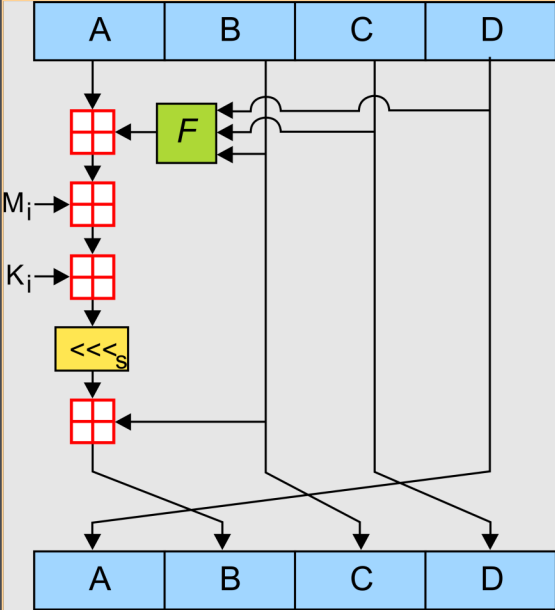
\includegraphics[width=0.4\textwidth]{figures/fig09-md5}
    \centering
    \caption{MD5 Operation, die 64 Mal wiederholt wird}
\end{figure}


\section{SHA (Secure Hash Algorithm)}\index{Hashfunktion!SHA}\index{SHA}

1993 wurde SHA-0 veröffentlicht, 1995 dann der verbesserte SHA-1 und 2001 SHA-2. Das NIST hat SHA-3 ausgeschrieben, das Ende des Auswahlprozesses war 2012 (vgl. AES).
Dann wurde Keccak als SHA-3 2015 standardisiert. \\

\paragraph{SHA-1}\index{SHA-1}
Der SHA-1 mit voller Rundenzahl gilt seit 2005 als unsicher. Kollisionen können mit $2^{63}$ Operationen erzeugt werden, 2008 wurde die Zahl auf $2^{51}$ verringert.
Seit 2017 sind Kollisionen in 2 validen PDF Dokumenten konstruierbar. \\

Er erzeugt einen 160 Bit Output und basiert auf denselben Grundideen wie MD4 und MD5:

\begin{itemize}
    \item Nachricht ebenfalls in 512-Bit Blöcke gespalten
    \item es gibt 80 Runden, alle 20 Runden wechselt die Rundenfunktion
    \begin{enumerate}
        \item F(X,Y,Z) = (X and Y) or (not X and Z) (ident zu MD5)
        \item G(X,Y,Z) = X $\oplus$ Y $\oplus$ Z (ident zu H aus MD5)
        \item H(X,Y,Z) = (X and Y) or (X and Z) or (Y and Z)
        \item I(X,Y,Z) = G (sic)
    \end{enumerate}
    \item es gibt 4 Rundenkonstanten
    \begin{enumerate}
        \item $K_1 = 230 \cdot \sqrt(2)$ 
        \item $K_2 = 230 \cdot \sqrt(3)$
        \item $K_3 = 230 \cdot \sqrt(5)$
        \item $K_4 = 230 \cdot \sqrt(10)$
    \end{enumerate}
    \item In jeder Runde um 30 zirkulär geshiftet
\end{itemize}

\paragraph{SHA-2}\index{SHA-2} beschreibt eine Familie an Hashfunktionen, die die Algorithmen SHA-224, SHA-256, SHA-384, SHA-512, SHA-512/224 und SHA-512/256. Sie sind im 
FIPS 
(Federal Information Processing Standards) PUB-180-4 beschrieben.


\begin{center}
    \begin{tabular}{ llll } 
        \hline
        Algorithmus & Ausgabegröße (Bit) & Interne Blockgröße (Bit) & basiert auf \\ 
        \hline
        SHA-224     & 224 &  512 & SHA-256\\
        SHA-256     & 256 &  512 & SHA-256\\
        SHA-384     & 384 & 1024 & SHA-512\\
        SHA-512     & 512 & 1024 & SHA-512\\
        SHA-512/224 & 224 & 1024 & SHA-512\\
        SHA-512/256 & 256 & 1024 & SHA-512\\
        \hline
    \end{tabular}
\end{center}

\subparagraph{SHA-224}: Kürzere Version von SHA-256 mit 224 Bit Ausgabelänge. Geeignet, wenn Speicher knapp ist, z.B. constraint devices (Memory).
\subparagraph{SHA-256}: Der meistverwendete SHA-2-Algorithmus. Standard für viele Anwendungen (z. B. TLS, digitale Signaturen)
\subparagraph{SHA-384}: Abgespeckte Version von SHA-512 mit anderer Initialisierung und kürzerer Ausgabe.
\subparagraph{SHA-512}: Sicherste (längste) Standardvariante mit 512 Bit Ausgabelänge.
\subparagraph{SHA-512/224} (constraint devices (Memory)), siehe SHA-512/256.  
\subparagraph{SHA-512/256} (allg. Sicherheit): Truncate-Versionen von SHA-512 mit kürzerer Ausgabelänge. Bietet eine Kombination aus höherer
Sicherheit (wegen 1024-Bit Blockgröße) und kürzeren Hashes.


\subparagraph{Merkle-Damgard}\index{Merkle-Damgard}\index{Hashfunktion!Merkle-Damgard}

Die Merkle-Damg\r{a}rd-Konstruktion (auch Merkles Meta-Verfahren) ist eine Methode zur Konstruktion von kryptographischen Hash-Funktionen, die auf Arbeiten von 
Ralph Merkle und Ivan Damg\r{a}rd zurückgeht.
Gegeben ist eine kollisionsresistente Kompressionsfunktion $f: \{0, 1\}^{a+b} \to \{0, 1\}^b$. Durch die Anwendung der Merkle-Damg\r{a}rd-Konstruktion ergibt sich daraus 
eine kollisionssichere Hash-Funktion $h: \{0, 1\}^* \to \{0, 1\}^b$, die beliebig lange Nachrichten auf einen Hashwert abbilden.

\begin{figure}[h]
    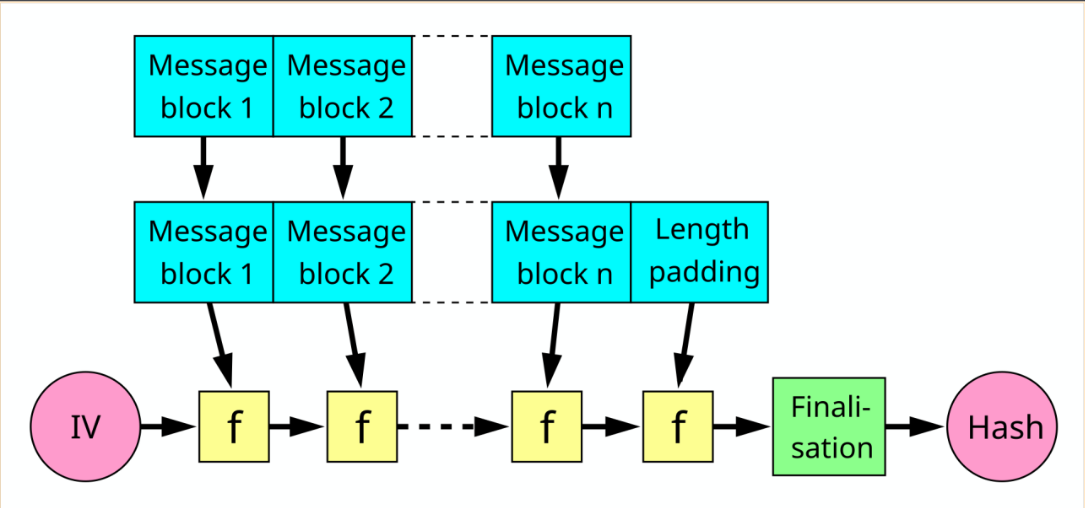
\includegraphics[width=0.9\textwidth]{figures/fig10-merkle-damgard}
    \centering
    \caption{Merkle-Damgard Hash}
\end{figure}

\begin{enumerate}
    \item Padding (Auffüllen): Die Eingabenachricht wird so erweitert, dass ihre Länge ein Vielfaches der Blockgröße ist. Dabei wird meist die ursprüngliche 
    Nachrichtenlänge am Ende angehängt.
    \item Aufteilung in Blöcke: Die aufgefüllte Nachricht wird in gleichgroße Blöcke unterteilt.
    \item Initialisierung: Ein fester Startwert (IV = Initialization Vector) wird gesetzt.
    \item Iterative Verarbeitung: Für jeden Block wird die Kompressionsfunktion angewendet:
    \begin{itemize}
        \item Eingabe: der aktuelle Block + der Ausgabewert des vorherigen Schritts
        \item Ausgabe: ein neuer Zwischenwert
    \end{itemize}
    \item Finales Ergebnis: Der Ausgabewert nach dem letzten Block ist der Hash-Wert.
\end{enumerate}

\subsection{SHA-3}\index{SHA-3}

2007 begann das NIST mit der Ausschreibung für einen Nachfolger von SHA-2. Am 2.10.2012 wurde Keccak (von Guido
Bertoni, Joan Daemen, Gilles Van Assche und Michaël Peeters) als Sieger verkündet und stellt die Basis für SHA-3 dar.

\begin{itemize}
    \item Verwendet im Unterschied zur bisherigen SHA Familie eine sog. ``Sponge'' Konstruktion: ein 3-dimensionaler innerer Zustand ($5\times 5\times w$ -Bit Wörter; 
    bei $w =64$ sind das 1.600 Bits)
    \item Permutation: 24 Runden, 5 Schritte ($\theta, \rho, \pi, \chi, \iota$)
    \item Zuerst wird der zu hashende Text zur Gänze ``aufgesogen'' (absorbing phase)
    \item Danach der Hash gewünschter Länge ``ausgepresst'' (squeezing phase)
    \item Das ergibt Hashlängen von 224 bis 512 Bit (theoretisch aber beliebig lange, bis maximal 1.600); wird auch als Capacity Wert bezeichnet
\end{itemize}

\paragraph{Phasen}

\begin{figure}[h]
    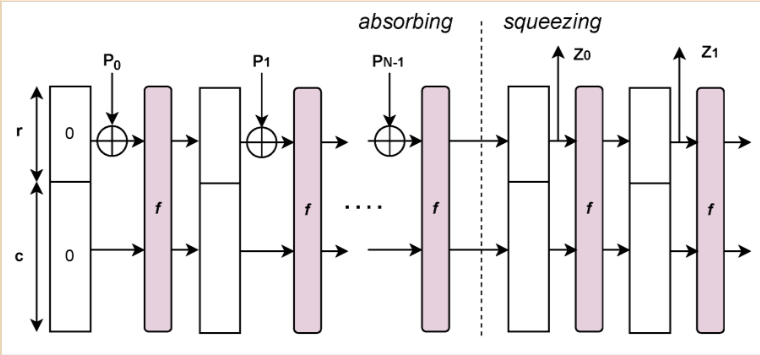
\includegraphics[width=0.75\textwidth]{figures/fig11-sponge}
    \centering
    \caption{SHA-3, Absorbing- und Squeezing Phase}
\end{figure}

\subparagraph{Absorbieren} Eingabedaten werden in Blöcke unterteilt.
Jeder Block wird mit dem internen Zustand (einer Art Speicher) verXORt.
Danach wird eine Permutation ($f$) auf den Zustand angewendet.

\subparagraph{Auspressen} Nachdem alle Eingabeblöcke
absorbiert wurden, wird ein Teil des internen Zustands als Ausgabe extrahiert.
Bei langen Ausgaben (z.B. SHAKE-Funktionen) wird $f$ mehrfach ausgeführt, um mehr Output zu generieren.

\paragraph{State} Der interne Zustand in KECCAK hat die Breite $b=1600$ Bits (für SHA-3). Dieser Zustand ist aufgeteilt in ein 3D-Array mit
Dimensionen $5 \times 5 \times w$, wobei $w = 64$ bits. Jede Zelle $A[x][y]$ ist ein sogenanntes ``lane'' mit 64 Bits. 

\paragraph{Parameter}

Neben der Größe des States $b$, gibt es noch die Parameter

\begin{itemize}
    \item Rate $r$, wie viele Bits pro Sekunde verarbeitet werden können 
    \item Capacity $c$, wie groß die Sicherheitsreserve ist, sie berechnet sich als $c = b - r$. Bei Kapazität $c$  bietet der Algorithmus $c/2$ Bit Widerstand gegen 
    Kollisions- und Preimage-Attacken. 
\end{itemize}

Für den SHA-256 haben die Parameter $(b, r, c)$ dem Wert $(1600, 1088, 512)$.

\paragraph{Permutationsfunktion} KECCAK-f hat 24 Runden mit je 5 Steps:
\begin{enumerate}
    \item $\theta$ (theta) mischt jede Lane mit einer XOR-Mischung ihrer Spaltennachbarn.
    \item $\rho$ (rho) rotiert die Bits jeder Lane um einen bestimmten Wert.
    \item $\pi$ (pi) permutiert die Positionen der Lanes im $5\times 5$-Gitter.
    \item $\chi$ (chi) führt eine nichtlineare XOR-Maske aus, basierend auf anderen Werten in der Zeile.
    \item $\iota$ (iota) fügt einen Rundenkonstanten hinzu (zum Schutz vor symmetrischen Mustern).
\end{enumerate}

\noindent Diese Schritte garantieren Diffusion, Konfusion und Nichtlinearität, wie bei modernen
Blockchiffren.

\paragraph{Padding} Um sicherzustellen, dass die Nachricht gleichmäßig in $r$-Bit-Blöcke aufgeteilt werden
kann, ist ein Padding erforderlich. SHA-3 verwendet das Muster 100...001 (01 Padding), ein Bit mit Wert 1 wird gefolgt von null oder mehr 0-Bits (maximal $r-1$) und 
einem letzten 1-Bit.

\paragraph{XOFs} (Extendable Output Functions) basieren auf KECCAK und geben beliebig viele Ausgabebits zurück (nicht nur 256 oder 512).
Sie sind sehr flexibel für Anwendungen wie:
\begin{itemize}
    \item Key Derivation Function (KDF)
    \item Authentifizierung
    \item PQC Signaturen (z. B. SPHINCS+, Dilithium)
\end{itemize}

SHAKE bezeichnet den KECCAK Algorithmus, der er ein anderes Padding (1111 statt 01) und eine variable Ausgabelänge hat.


\section{Angriffe}\index{Hashfunktion!Angriffe}\index{Angriffe!Hashfunktion}

Sei $n$ die Länge des Outputs. Die Angriffe auf Hashfunktionen können wie folgt kategorisiert werden:

\begin{itemize}
    \item Angriff auf die Eigenschaft als Einwegfunktion: Idealerweise Komplexität von $O(2^n)$
    \item Angriff auf die schwache Kollisionsresistenz: Idealerweise Komplexität von $O(2^n)$ 
    \item Angriff auf die starke Kollisionsresistenz: Idealerweise Komplexität von $1.2\cdot 2^{n/2}$ (Geburtstagsparadoxon)
\end{itemize}

Generell gilt, ein Aufwand von $2^{80}$ ist ``schwierig''.

\paragraph{MD5} ist gebrochen.
\paragraph{SHA-1} ist gebrochen.
\paragraph{SHA-2} 

\begin{itemize}
    \item Output: 224/256/384/512 Bit
    \item Struktur: Merkle-Damgard
    \item Theoretische Angriffe auf rundenreduzierte Versionen bekannt
\end{itemize}

\paragraph{SHA-3}

\begin{itemize}
    \item Output: 224/256/384/512 Bit
    \item Struktur: Sponge
\end{itemize}

\subsection{BEAST Attack}

Steht für \textbf{B}rowser \textbf{E}xploit \textbf{A}gainst \textbf{S}SL/\textbf{T}LS.
\begin{itemize}
    \item MitM Angriff und Chosen Plaintext Attack
    \item Record Splitting
    \item CBC Mode mit unsicherer IV-Generierung
    \item Beschrieben in CVE-2011-3389
    \item TLS1.0
\end{itemize}

Der BEAST-Angriff nutzt die Tatsache aus, dass bei TLS 1.0 der
Initialisierungsvektor (IV) für die nächste Nachricht vorhersehbar ist:
Er ist nämlich der letzte verschlüsselte Block der vorherigen Nachricht.

Dadurch kann ein Angreifer über sogenannte Chosen-Plaintext-Angriffe (d. h. gezielt eingefügte Daten) Rückschlüsse auf vertrauliche
Inhalte wie Cookies ziehen. \\

\noindent Damalige temporäre Workarounds
\begin{itemize}
    \item RC4
    \item 0-length Packets
    \item 1/n-1 Packet-Splitting: 
    \begin{itemize}
        \item Erster Record (1 Byte): Enthält nur ein harmloses Byte (z. B. ein Leerzeichen oder ein kontrolliertes Zeichen).
        \item Zweiter Record (n-1 Bytes): Enthält den Rest der eigentlichen Nachricht (z.B. HTTP-Headers, Cookies usw.).
    \end{itemize}
\end{itemize}
 

\begin{figure}[h]
    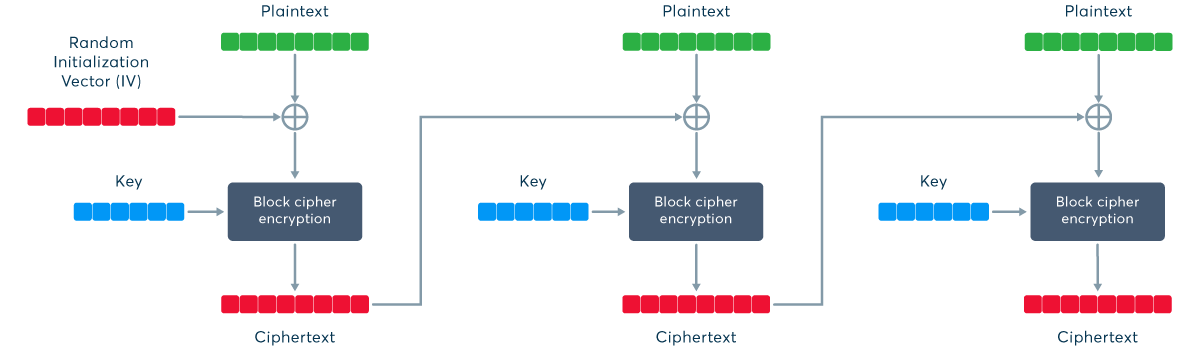
\includegraphics[width=0.9\textwidth]{figures/fig12-beast-attack-1}
    \centering
    \caption{How it should work: Proper encryption using a block cipher in CBC mode}
\end{figure}
\begin{figure}[h]
    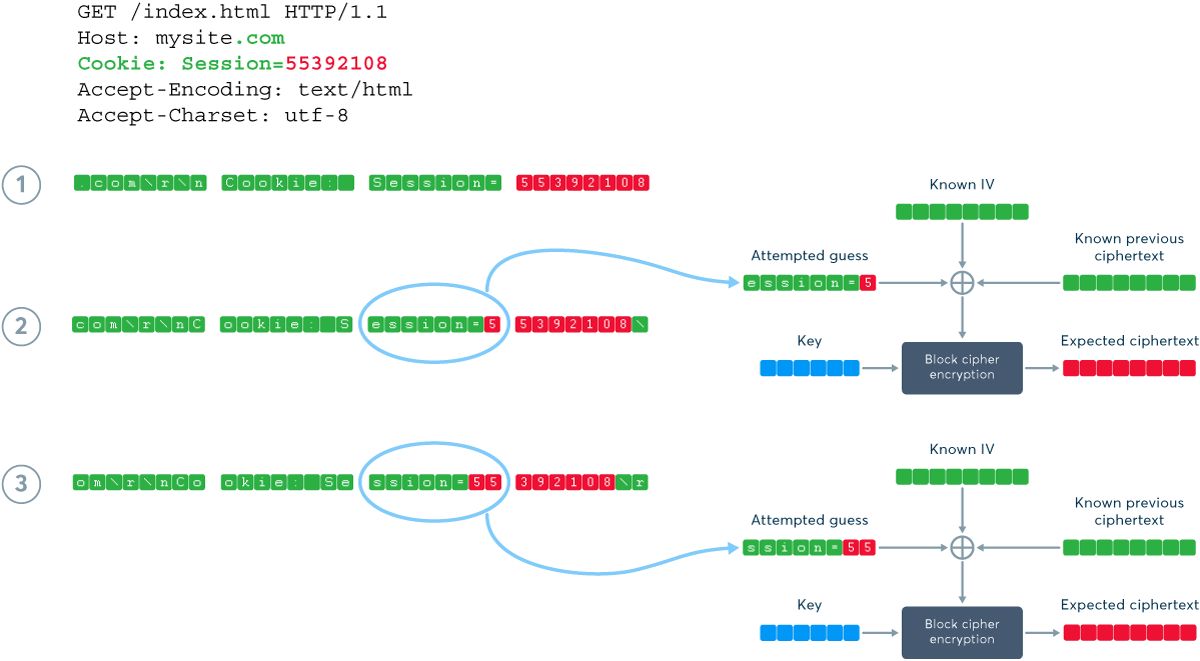
\includegraphics[width=0.9\textwidth]{figures/fig13-beast-attack-2}
    \centering
    \caption{The underlying vulnerability: A record splitting attack against TLS 1.0}
\end{figure}
\begin{figure}[h]
    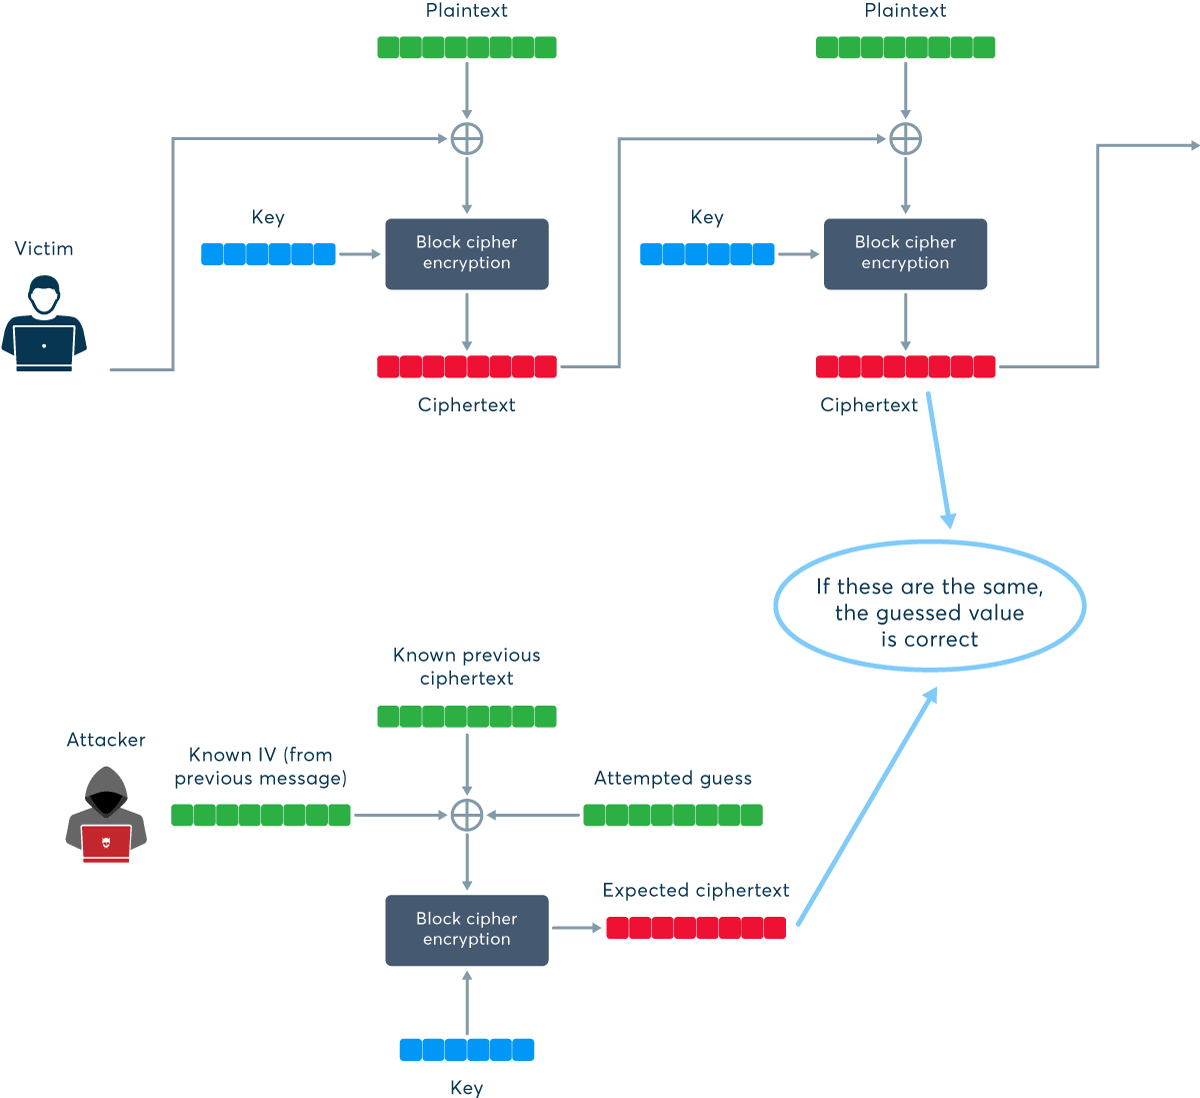
\includegraphics[width=0.9\textwidth]{figures/fig14-beast-attack-3}
    \centering
    \caption{The BEAST exploit: A chosen boundary attack combined with record splitting}
\end{figure}
\input{chapters/7-integer-factorisation}
\input{chapters/8-signatures}

%%% backmatter %%%
\backmatter

% \bibliographystyle{plain}
% \bibliography{bibliography}
\printindex

\end{document}

